%!TEX root = ../../thesis.tex

Soon we will see how double layers can be used to perform electrical work.
Doing so relies specifically on the formation of double layers on insulating surfaces like glass.
Part \ref{part:doubleLayersOnInsulators} studies interfacial double layers on insulators.

It was discussed in the introduction that double layers naturally form at liquid-solid interfaces.
It was said that the double layer itself is a collection of charged ions.
Can we collect this charge and use it to generate electrical power?
Doing so would provide a method of energy harvesting without moving parts.
I look at a smart application of a water such a harvester, create a power budget, and discuss the design of a practical harvester.

\chapter{Introduction}
  \label{chap:harvesterIntroduction}
  This introductory chapter provides background reading specific to energy harvesting.
  It builds upon the preceding introductory material of double layers and is steered toward energy conversion.
  Here we are concerned with double layer formation on solid boundaries that are non-conducting, such as glass.
  We will discuss how this can be used to convert fluid-mechanical power into electrical power.
  At this point it is assumed the reader knows what a double layer is and how they are formed.

  \section{Streaming Cell Principle}

    % \begin{figure}
    %     \centering
    %     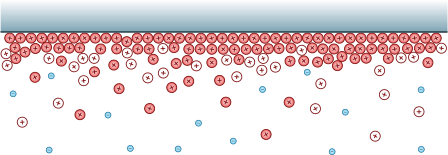
\includegraphics{content/pt1/01-PowerHarvesting/graphics/doubleLayerOnWall}
    %     \caption{\label{fig:doubleLayerOnWall}A double layer formed on a wall}
    % \end{figure}
    \begin{figure}
        \centering
        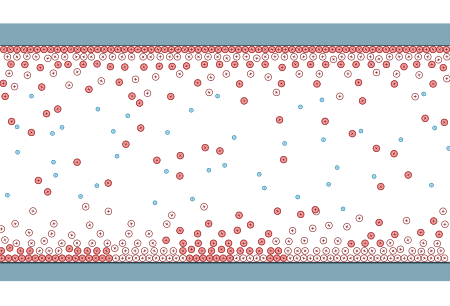
\includegraphics{content/pt1/01-PowerHarvesting/graphics/intro_walls}
        \caption{\label{fig:doubleLayerBetweenWalls}Formation of a double layer between two  walls}
    \end{figure}

    Lets begin by looking at double layers that have formed along the walls of a container.
    Such a situation is presented in \ref{fig:doubleLayerBetweenWalls}, where the walls are negatively charged and the counter-ions are positive.
    The counter-ions line the interior walls of the container.
    The charge density at the walls is higher than in the bulk of the solution, owing to charge separation within the liquid.
    However, charge separation is not enough to generate electrical power.

    Electrical power can not be drawn directly from the charged layer because:
    \begin{itemize}
        \item The counter-ions are electrostatically bound to the interface.
            Removing these ions from the interface requires work.
        \item Charge migration, from the fluid bulk into the layer, stops once the layer has neutralised the surface charge at the interface.
    \end{itemize}
    But, the layer can be used as a means of converting fluid energy into electrical energy.
    The means to do this lies in the use of suitable channels that separate two bodies of liquid.
    Such a channel is presented in figure \ref{fig:doubleLayerInChannel_noPressure}.

    \begin{figure}
        \centering
        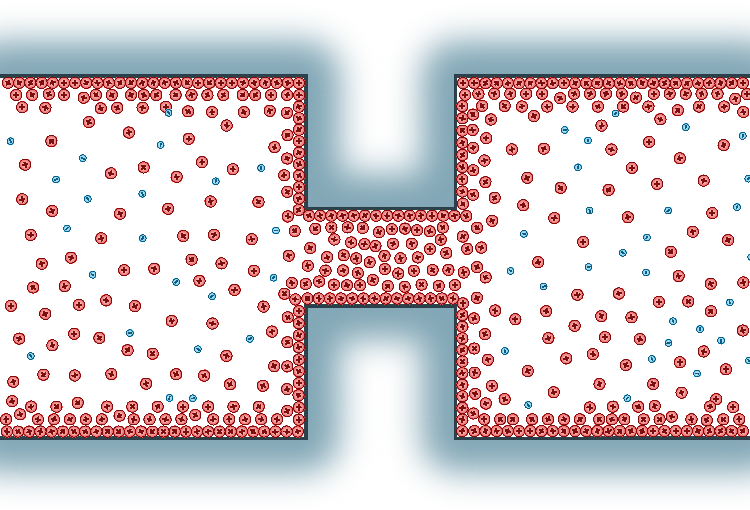
\includegraphics{content/pt1/01-PowerHarvesting/graphics/intro_cell_settled}
        \caption{\label{fig:doubleLayerInChannel_noPressure}Double layer formation within a cell geometry}
    \end{figure}

    Under static conditions the channels usefulness is not totally apparent.
    The two bodies separated by the channel are still similar in composition to the body presented in the previous figure.
    Importantly, the channel that lies between the two bodies contains a very high concentration of counter-ions.
    This is due to the channels height being in the order of the thickness of the double layer.

    % As two double layers are bought together co-ions within the fluid are repelled from the space between them.
    % There comes a point where the double layers being to overlap.
    % At this point 
    % The channel is now almost exclusively occupied by counter-ions, and the channel will oppose the entry of co-ions.
    % What has been created is a channel that will favour the transport of counter-ions over co-ions.

    \begin{figure}
        \centering
        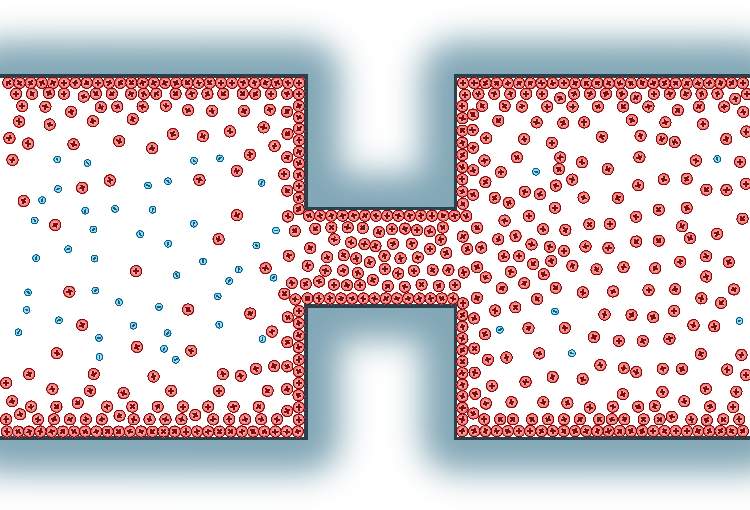
\includegraphics{content/pt1/01-PowerHarvesting/graphics/intro_cell_pressure}
        \caption{\label{fig:doubleLayerInChannel_pressure}Double layer formation in a cell geometry with the application of pressure}
    \end{figure}

    With the application of hydrostatic pressure across the channel, the contents of the channel moves toward the body with the lower pressure.
    More counter-ions move from the high pressure body into the channel to replenish the double layer.
    The pressure applied is now pumping charge between the bodies.




    % \begin{figure}
    %   \centering
    %     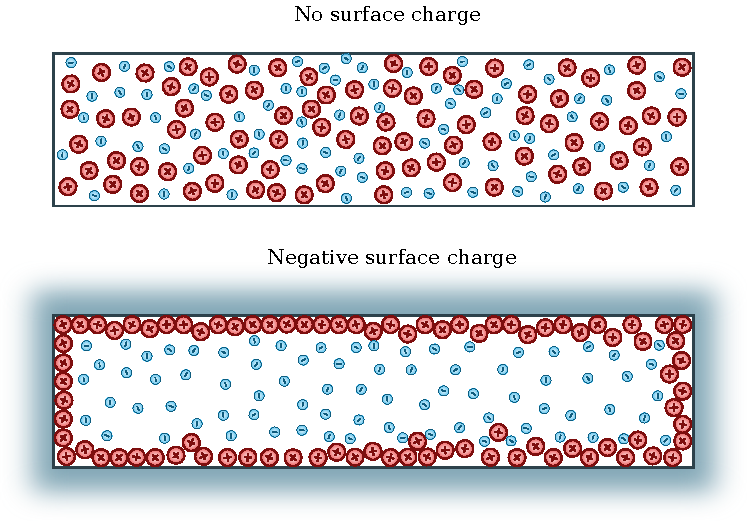
\includegraphics{content/pt1/01-PowerHarvesting/graphics/ionsInABox.pdf}
    %     \caption{\label{fig:ionsInABox}Charge distribution in a charged cavity versus a non-charged cavity}
    % \end{figure}

    % Now imagine a very small cavity filled with an electrolyte.
    % A simplified representation of such a cavity is shown in figure \ref{fig:ionsInABox}.
    % If the walls of the cavity hold no surface charge then the ions distribute evenly throughout the volume.
    % That is to say, the ions in the liquid are not electrically influenced by the walls.
    % With the application of surface charge - the counter-ions migrate to the walls.
    % As the density of counter-ions has increased at the interface, a void of cations remains within the cavity.
    % The charge has been separated.



    Now lets imagine bringing another wall in toward the first (as shown in figure~\ref{fig:doubleLayerBetweenWalls}).
    By controlling the thickness of the double layer and the distance between the walls, it is possible to overlap the double layers.
    Bringing these walls together acts to repel any co-ions from between the walls.
    Removing the co-ions increases the counter-ion concentration with the body of liquit between the walls

    Double layers are usually very thin, in the order of nanometers, so overlapping them requires very small geometries.
    Geometries formed for this purpose are very narrow channels, whose walls contain trapped charge.

    


    



    % A streaming potential is simply a very thin cavity separating two volumes.
    % The walls of the cavity are separated by a distance in the order of a couple of double layers.
    % These dimensions are such that double layers within the cavity overlap.
    % By overlapping double layers, the volume of liquid within the cavity is primarily comprised of double layer counter-ions.

    % The streaming potential cell is a device that uses water flow to separate charge.
    % It is particularly promising as a harvester due to its lack of moving parts.
    % This chapter starts by explaining how a streaming cell makes use of the interfacial double layer to separate charge.
    % Then I construct a crude cell and measure its performance.
    % This is followed by a mathematical investigation of the streaming cell.

    % For the sake of brevity, the term `cell' in this chapter shall refer to a streaming potential cell.
    % And the term `interface' refers to the interface, or boundary, between solid and liquid matter.
    % Unless otherwise stated, it should be assumed that I am describing the liquid side of the interface.
    % The solid body typically plays no role, apart from the surface charge it holds.

    % \begin{figure}
    %     \centering
    %     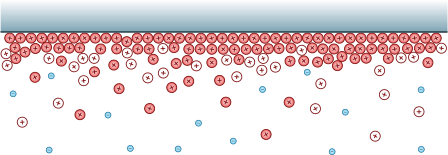
\includegraphics{content/pt1/01-PowerHarvesting/graphics/doubleLayerOnWall}
    %     \caption{\label{fig:doubleLayerOnWall}Formation of a double layer on a wall}
    % \end{figure}

    % Figure \ref{fig:doubleLayerOnWall} shows the formation of a double layer at the interface of a charged wall.
    % A higher density of positively charged ions, or cations, sit close to the interface.
    % The density of these cations reduces as the distance to the interface increases.
    % Also, the density of negatively charged ions, or anions, increases with the distance from the interface.


    To cause continuous charge separation, the cell is placed across a pressure gradient.
    This pressure gradient causes the counter-ions within the cavity to be pumped through the cell.
    As counter-ions are moved through the cavity, more counter-ions move to the replenish the layer at the opening.
    The counter-ions accumulate at the exit side of the cell.
    This scenario is illustrated in figure \ref{fig:streamingCellPrinciple}.

    Streaming potential cells are not new.
    They find use in collodial science as a means of measuring the zeta potential of a double layer \cite{Gu2000,Scales1992,Daiguji2004,VanderHeyden2006,Mala1997}.
    At the beginning of this work it was believed that harvesting power from streaming cells had not been done before.




    a cavity forcing water through narrow cavities. This phenomenon is understood
    and is used in colloidal science to determine what's called the zeta potential
    of an interface \cite{Gu2000,Scales1992,Daiguji2004,VanderHeyden2006,Mala1997}.
    Although this phenomenon isn't new, using it to generate useful amounts of
    electrical energy is. This chapter will investigate the application of
    streaming potentials to energy harvesting for the purposes of running a smart
    water meter.

    % At the boundary between a liquid and a solid, be it a molecule or the wall of
    % a container, there is a possibility for an electrical potential. This
    % electrical potential exists at the interface between the liquid and the solid
    % and is the underlying mechanism by which the streaming potential cell
    % operates. To understand how this electrical potential is able to separate
    % charge as it does in a streaming potential cell we will first observe what
    % happens when a solid suspended in liquid, as is shown in Figure
    % \ref{Figure_Diagram_ZetaPotential_and_SlippingPlane}.


    \begin{figure} \centering
        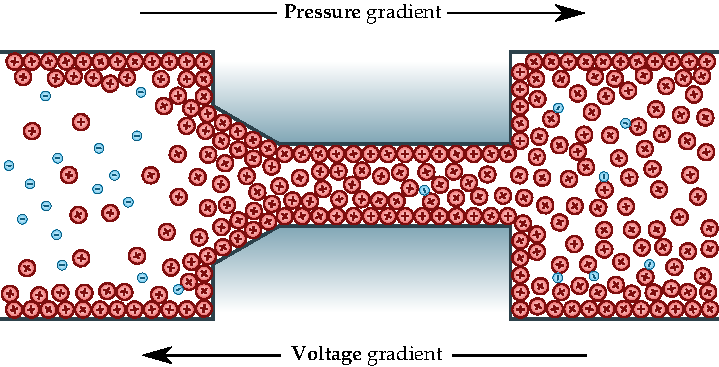
\includegraphics{content/pt1/01-PowerHarvesting/graphics/streamingCellPrinciple}
        \caption{\label{fig:streamingCellPrinciple}The general principle of
            operation of the streaming potential cell} \end{figure} In this
    diagram, a the negatively charged solid is surrounded by layers of positively
    charged ions that are electrostaticly attracted to the surface of the solid.
    Near the surface of the solid, tightly bound, positively charged ions are
    packed together and are largely immobile.  These ions reside in what is called
    the Stern Layer. After this layer is a shell of less densely packed and
    somewhat mobile ions that are still bound to the solid. At the edge of this
    shell is what is called the slipping plane, which is the point at which ions
    are no-longer bound to the solid. The electrical potential at this slipping
    plane is termed the $\zeta$ potential (zeta potential). ``This zeta potential
    is directly related to the interaction between the solid particles themselves
    when they are suspended in a liquid and thus determines the stability of the
    suspension solutions'' \cite{Gu2000}.

    % \begin{figure} \begin{centering}
    % 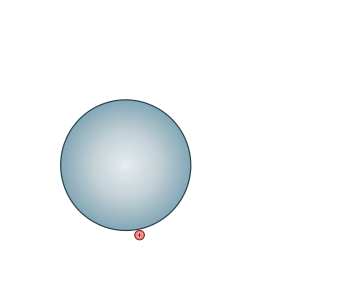
\includegraphics[scale=0.12]{content/pt1/01-PowerHarvesting/Diagram_of_zeta_potential_and_slipping_plane_thesisEdit}
    % \par\end{centering}

    % \centering{}\protect\caption{\label{Figure_Diagram_ZetaPotential_and_SlippingPlane}Diagram
    % showing the ionic concentration and potential difference as a function of
    % distance from the charged surface of a particle suspended in a dispersion
    % medium.} \end{figure}


    Now lets look at the case where the geometry is such that the surface charge
    resides on the walls of a channel through which the liquid can flow, as is
    shown in Figure \ref{Figure_Diagram_ZetaPotential_and_in_a_channel}.  By
    setting the width of the channel such that the double layer formed on each of
    the sides partially overlap, the channel will be predominantly occupied by ions
    of the opposite polarity to that of the surface charge at the solid to liquid
    interface. This configuration has the effect of promoting the transport of
    those ions across the channel with the application of a pressure differential
    across the channels length.

    %\begin{figure}
    %\centering{}\includegraphics[scale=0.12]{content/pt1/01-PowerHarvesting/Diagram_of_zeta_potential_in_a_channel_thesisEdit}\protect\caption{\label{Figure_Diagram_ZetaPotential_and_in_a_channel}Diagram
    %showing the ionic concentration and potential difference as a function of
    %distance from the charged surfaces of a micro-channel.} \end{figure}







  \section{Literature Review}

\chapter{The Streaming Cell Energy Harvester}
  \label{chap:harvestingEnergy}

  This chapter demonstrates an energy harvesting device capable of harvesting energy from flowing water with no moving parts.
  A `smart' use for such a harvester is discussed in chapter \ref{chap:wirelessWaterMetering}.
  I find the minimum power a harvester needs to harvest in order to be useful in chapter \ref{chap:energyRequirements}.
  And finally, in chapter \ref{chap:harvesterDesign}, I discuss the design of a harvester and comment on its feasibility.

  %!TEX root = ../../../thesis.tex

\section{The Streaming Potential Cell}
\label{sect:streamingPotentialCell}

The streaming potential cell is a device that uses water flow to separate charge.
It is particularly promising as a harvester due to its lack of moving parts.
This chapter starts by explaining how a streaming cell makes use of the interfacial double layer to separate charge.
Then I construct a crude cell and measure its performance.
This is followed by a mathematical investigation of the streaming cell.

For the sake of brevity, the term `cell' in this chapter shall refer to a streaming potential cell.
And the term `interface' refers to the interface, or boundary, between solid and liquid matter.
Unless otherwise stated, it should be assumed that I am describing the liquid side of the interface.
The solid body typically plays no role, apart from the surface charge it holds.

\begin{figure}
    \centering
    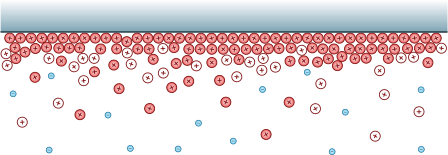
\includegraphics{content/pt1/01-PowerHarvesting/graphics/doubleLayerOnWall}
    \caption{\label{fig:doubleLayerOnWall}Formation of a double layer on a wall}
\end{figure}

Figure \ref{fig:doubleLayerOnWall} shows the formation of a double layer at the interface of a charged wall.
A higher density of positively charged ions, or cations, sit close to the interface.
The density of these cations reduces as the distance to the interface increases.
Also, the density of negatively charged ions, or anions, increases with the distance from the interface.

Now imagine a very small cavity filled with an electrolyte.
A simplified representation of such a cavity is shown in figure \ref{fig:ionsInABox}.
If the walls of the cavity hold no surface charge then the ions distribute evenly throughout the volume.
That is to say, the ions in the liquid are not electrically influenced by the walls.
With the application of surface charge - the counter-ions migrate to the walls.
As the density of counter-ions has increased at the interface, a void of cations remains within the cavity.
The charge has been separated.

\begin{figure}
    \centering
    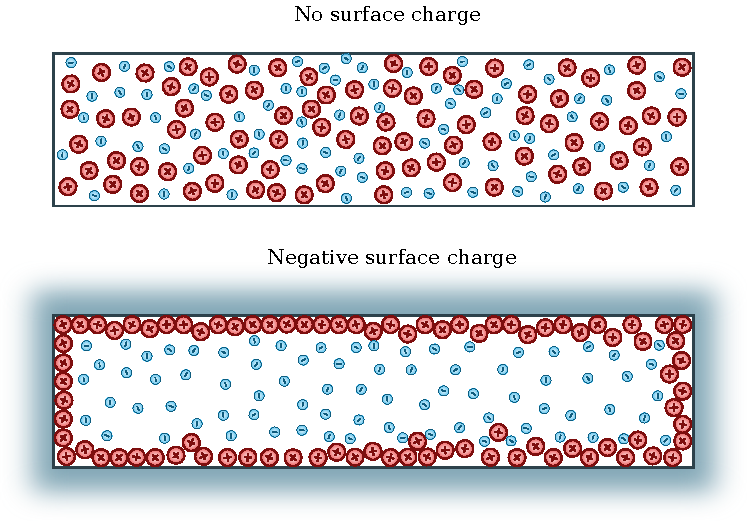
\includegraphics{content/pt1/01-PowerHarvesting/graphics/ionsInABox.pdf}
    \caption{\label{fig:ionsInABox}Charge distribution in a charged cavity versus a non-charged cavity}
\end{figure}

Charge separation is not enough to develop electrical power.
Electrical power can not be taken directly from a double layer because:
\begin{itemize}
    \item The counter-ions of a double layer are electrostatically bound to the interface.
        Removing these ions from the interface requires work.
    \item The double layer blocks the electric field from the interface.
        Charge migration stops once the layer has created an equal and opposite field at the interface.
\end{itemize}

A streaming potential is simply a very thin cavity separating two volumes.
The walls of the cavity are separated by a distance in the order of a couple of double layers.
These dimensions are such that double layers within the cavity overlap.
By overlapping double layers, the volume of liquid within the cavity is primarily comprised of double layer counter-ions.

To cause continuious charge separation, the cell is placed across a pressure gradient.
This pressure gradient causes the counter-ions within the cavity to be pumped through the cell.
As counter-ions are moved through the cavity, more counter-ions move to the replenish the layer at the opening.
The counter-ions accumulate at the exit side of the cell.
This scenario is illustrated in figure \ref{fig:streamingCellPrinciple}.

Streaming potential cells are not new.
They find use in collodial science as a means of measuring the zeta potential of a double layer \cite{Gu2000,Scales1992,Daiguji2004,VanderHeyden2006,Mala1997}.
At the beginning of this work it was believed that harvesting power from streaming cells had not been done before.




a cavity forcing water through narrow cavities. This phenomenon is understood
and is used in colloidal science to determine what's called the zeta potential
of an interface \cite{Gu2000,Scales1992,Daiguji2004,VanderHeyden2006,Mala1997}.
Although this phenomenon isn't new, using it to generate useful amounts of
electrical energy is. This chapter will investigate the application of
streaming potentials to energy harvesting for the purposes of running a smart
water meter.

% At the boundary between a liquid and a solid, be it a molecule or the wall of
% a container, there is a possibility for an electrical potential. This
% electrical potential exists at the interface between the liquid and the solid
% and is the underlying mechanism by which the streaming potential cell
% operates. To understand how this electrical potential is able to separate
% charge as it does in a streaming potential cell we will first observe what
% happens when a solid suspended in liquid, as is shown in Figure
% \ref{Figure_Diagram_ZetaPotential_and_SlippingPlane}.


\begin{figure} \centering
    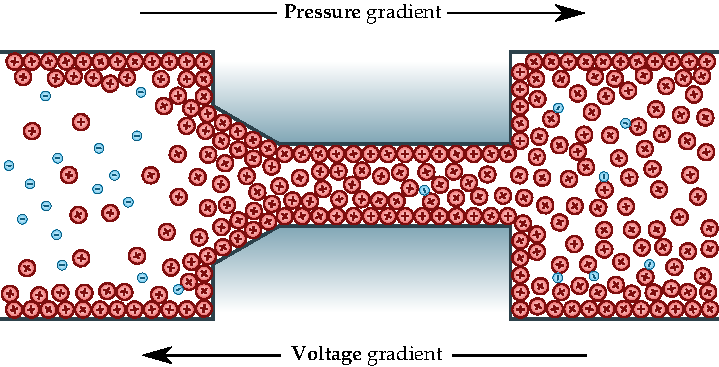
\includegraphics{content/pt1/01-PowerHarvesting/graphics/streamingCellPrinciple}
    \caption{\label{fig:streamingCellPrinciple}The general principle of
        operation of the streaming potential cell} \end{figure} In this
diagram, a the negatively charged solid is surrounded by layers of positively
charged ions that are electrostaticly attracted to the surface of the solid.
Near the surface of the solid, tightly bound, positively charged ions are
packed together and are largely immobile.  These ions reside in what is called
the Stern Layer. After this layer is a shell of less densely packed and
somewhat mobile ions that are still bound to the solid. At the edge of this
shell is what is called the slipping plane, which is the point at which ions
are no-longer bound to the solid. The electrical potential at this slipping
plane is termed the $\zeta$ potential (zeta potential). ``This zeta potential
is directly related to the interaction between the solid particles themselves
when they are suspended in a liquid and thus determines the stability of the
suspension solutions'' \cite{Gu2000}.

% \begin{figure} \begin{centering}
% 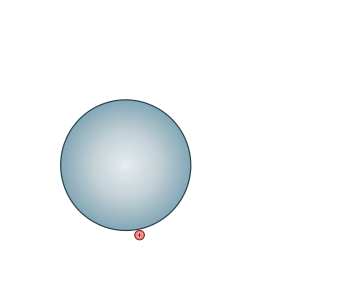
\includegraphics[scale=0.12]{content/pt1/01-PowerHarvesting/Diagram_of_zeta_potential_and_slipping_plane_thesisEdit}
% \par\end{centering}

% \centering{}\protect\caption{\label{Figure_Diagram_ZetaPotential_and_SlippingPlane}Diagram
% showing the ionic concentration and potential difference as a function of
% distance from the charged surface of a particle suspended in a dispersion
% medium.} \end{figure}


Now lets look at the case where the geometry is such that the surface charge
resides on the walls of a channel through which the liquid can flow, as is
shown in Figure \ref{Figure_Diagram_ZetaPotential_and_in_a_channel}.  By
setting the width of the channel such that the double layer formed on each of
the sides partially overlap, the channel will be predominantly occupied by ions
of the opposite polarity to that of the surface charge at the solid to liquid
interface. This configuration has the effect of promoting the transport of
those ions across the channel with the application of a pressure differential
across the channels length.

%\begin{figure}
%\centering{}\includegraphics[scale=0.12]{content/pt1/01-PowerHarvesting/Diagram_of_zeta_potential_in_a_channel_thesisEdit}\protect\caption{\label{Figure_Diagram_ZetaPotential_and_in_a_channel}Diagram
%showing the ionic concentration and potential difference as a function of
%distance from the charged surfaces of a micro-channel.} \end{figure}



\section{Replicating an Experiment}

There are many papers describing experiments with streaming potential cells
\cite{Gu2000,Mala1997,Scales1992,VanderHeyden2006} of which we have chosen one
by Yongan Gu and Dongqing Li \cite{Gu2000} to attempt to replicate. This paper
was chosen for its detailed description of the experimental procedure used,
including the brands and model numbers of the equipment used. Our experimental
procedure is based upon this paper however we have modified certain areas of
the experiment to accommodate for the resources available to us. For a list of
the materials used to construct the channels, see Table
\ref{Table_StreamingCell_MaterialsUsed}.


\subsection{\label{sub:Experimental-Procedure}Experimental procedure}


\subsubsection*{Construction}

\begin{figure}[p] \begin{centering}
        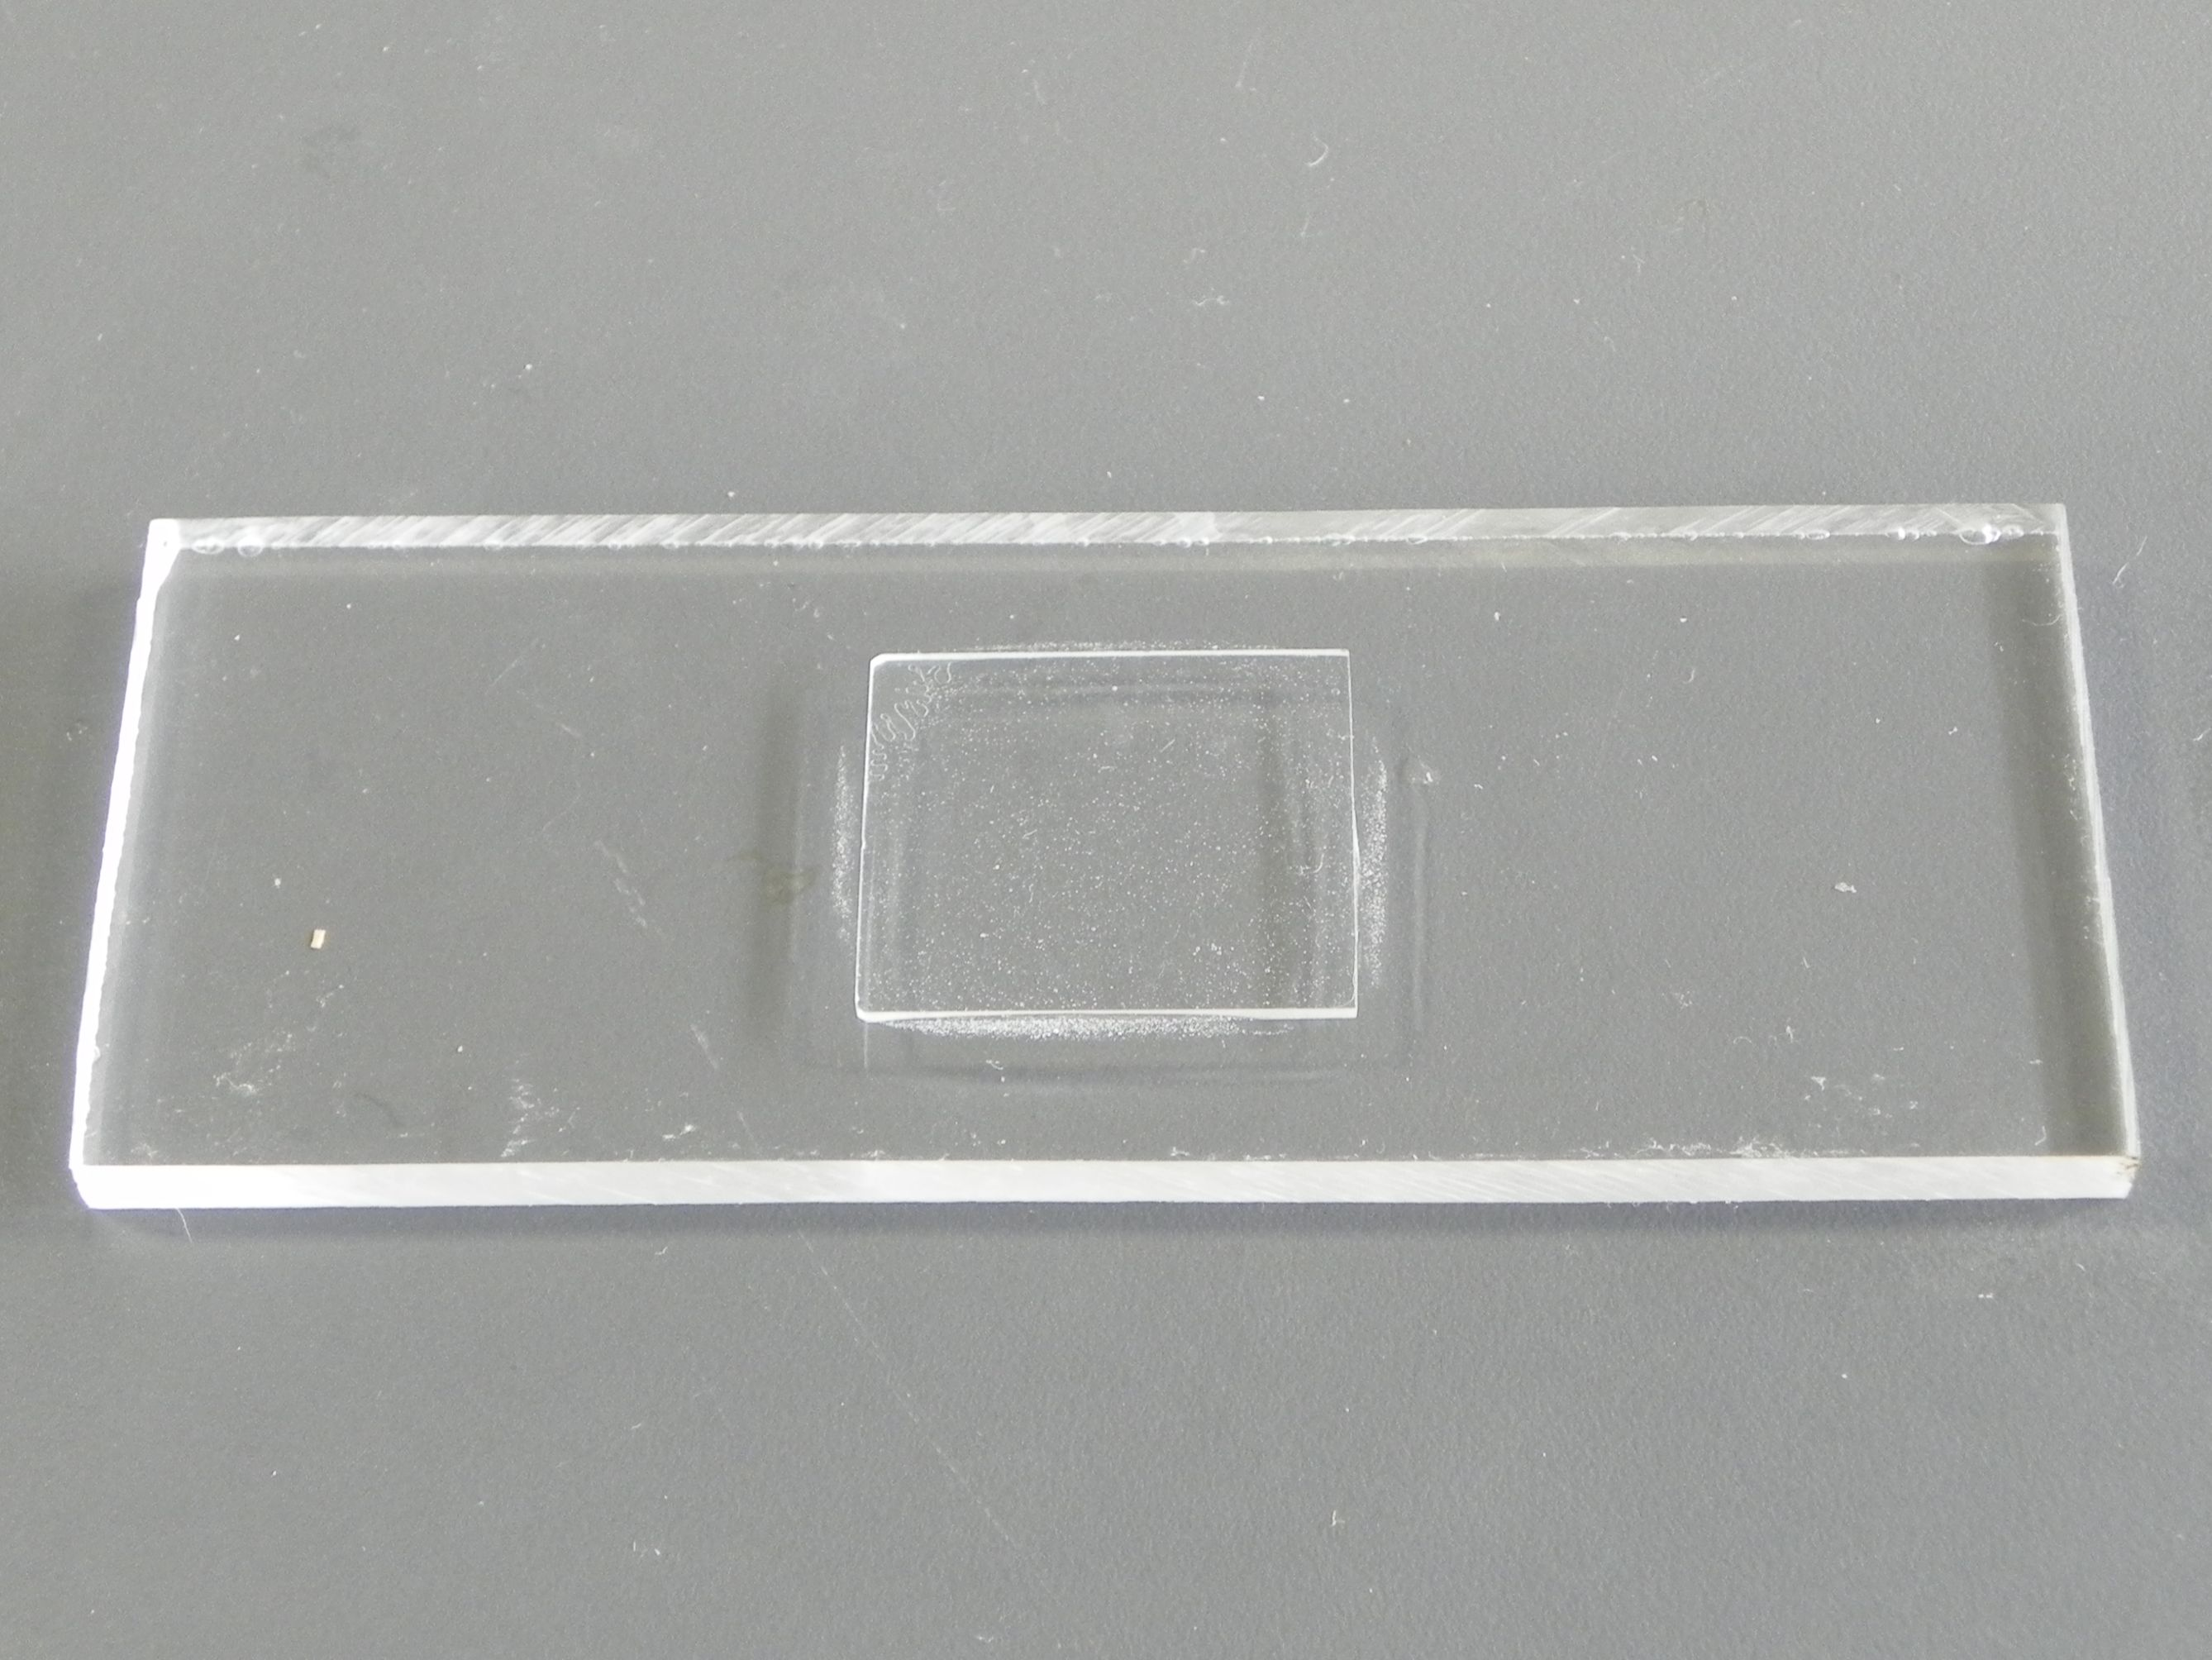
\includegraphics[width=0.5\textwidth]{content/pt1/01-PowerHarvesting/graphics/Photo_streamingPotential_Assembly_Step1.JPG}
        \par\end{centering}

\centering{}\protect\caption{\label{Photo_streamingPotential_Assembly_Step1}Photo
    showing half of a glass slide glued to acrylic base plate} \end{figure}
\begin{figure}[p] \begin{centering}
        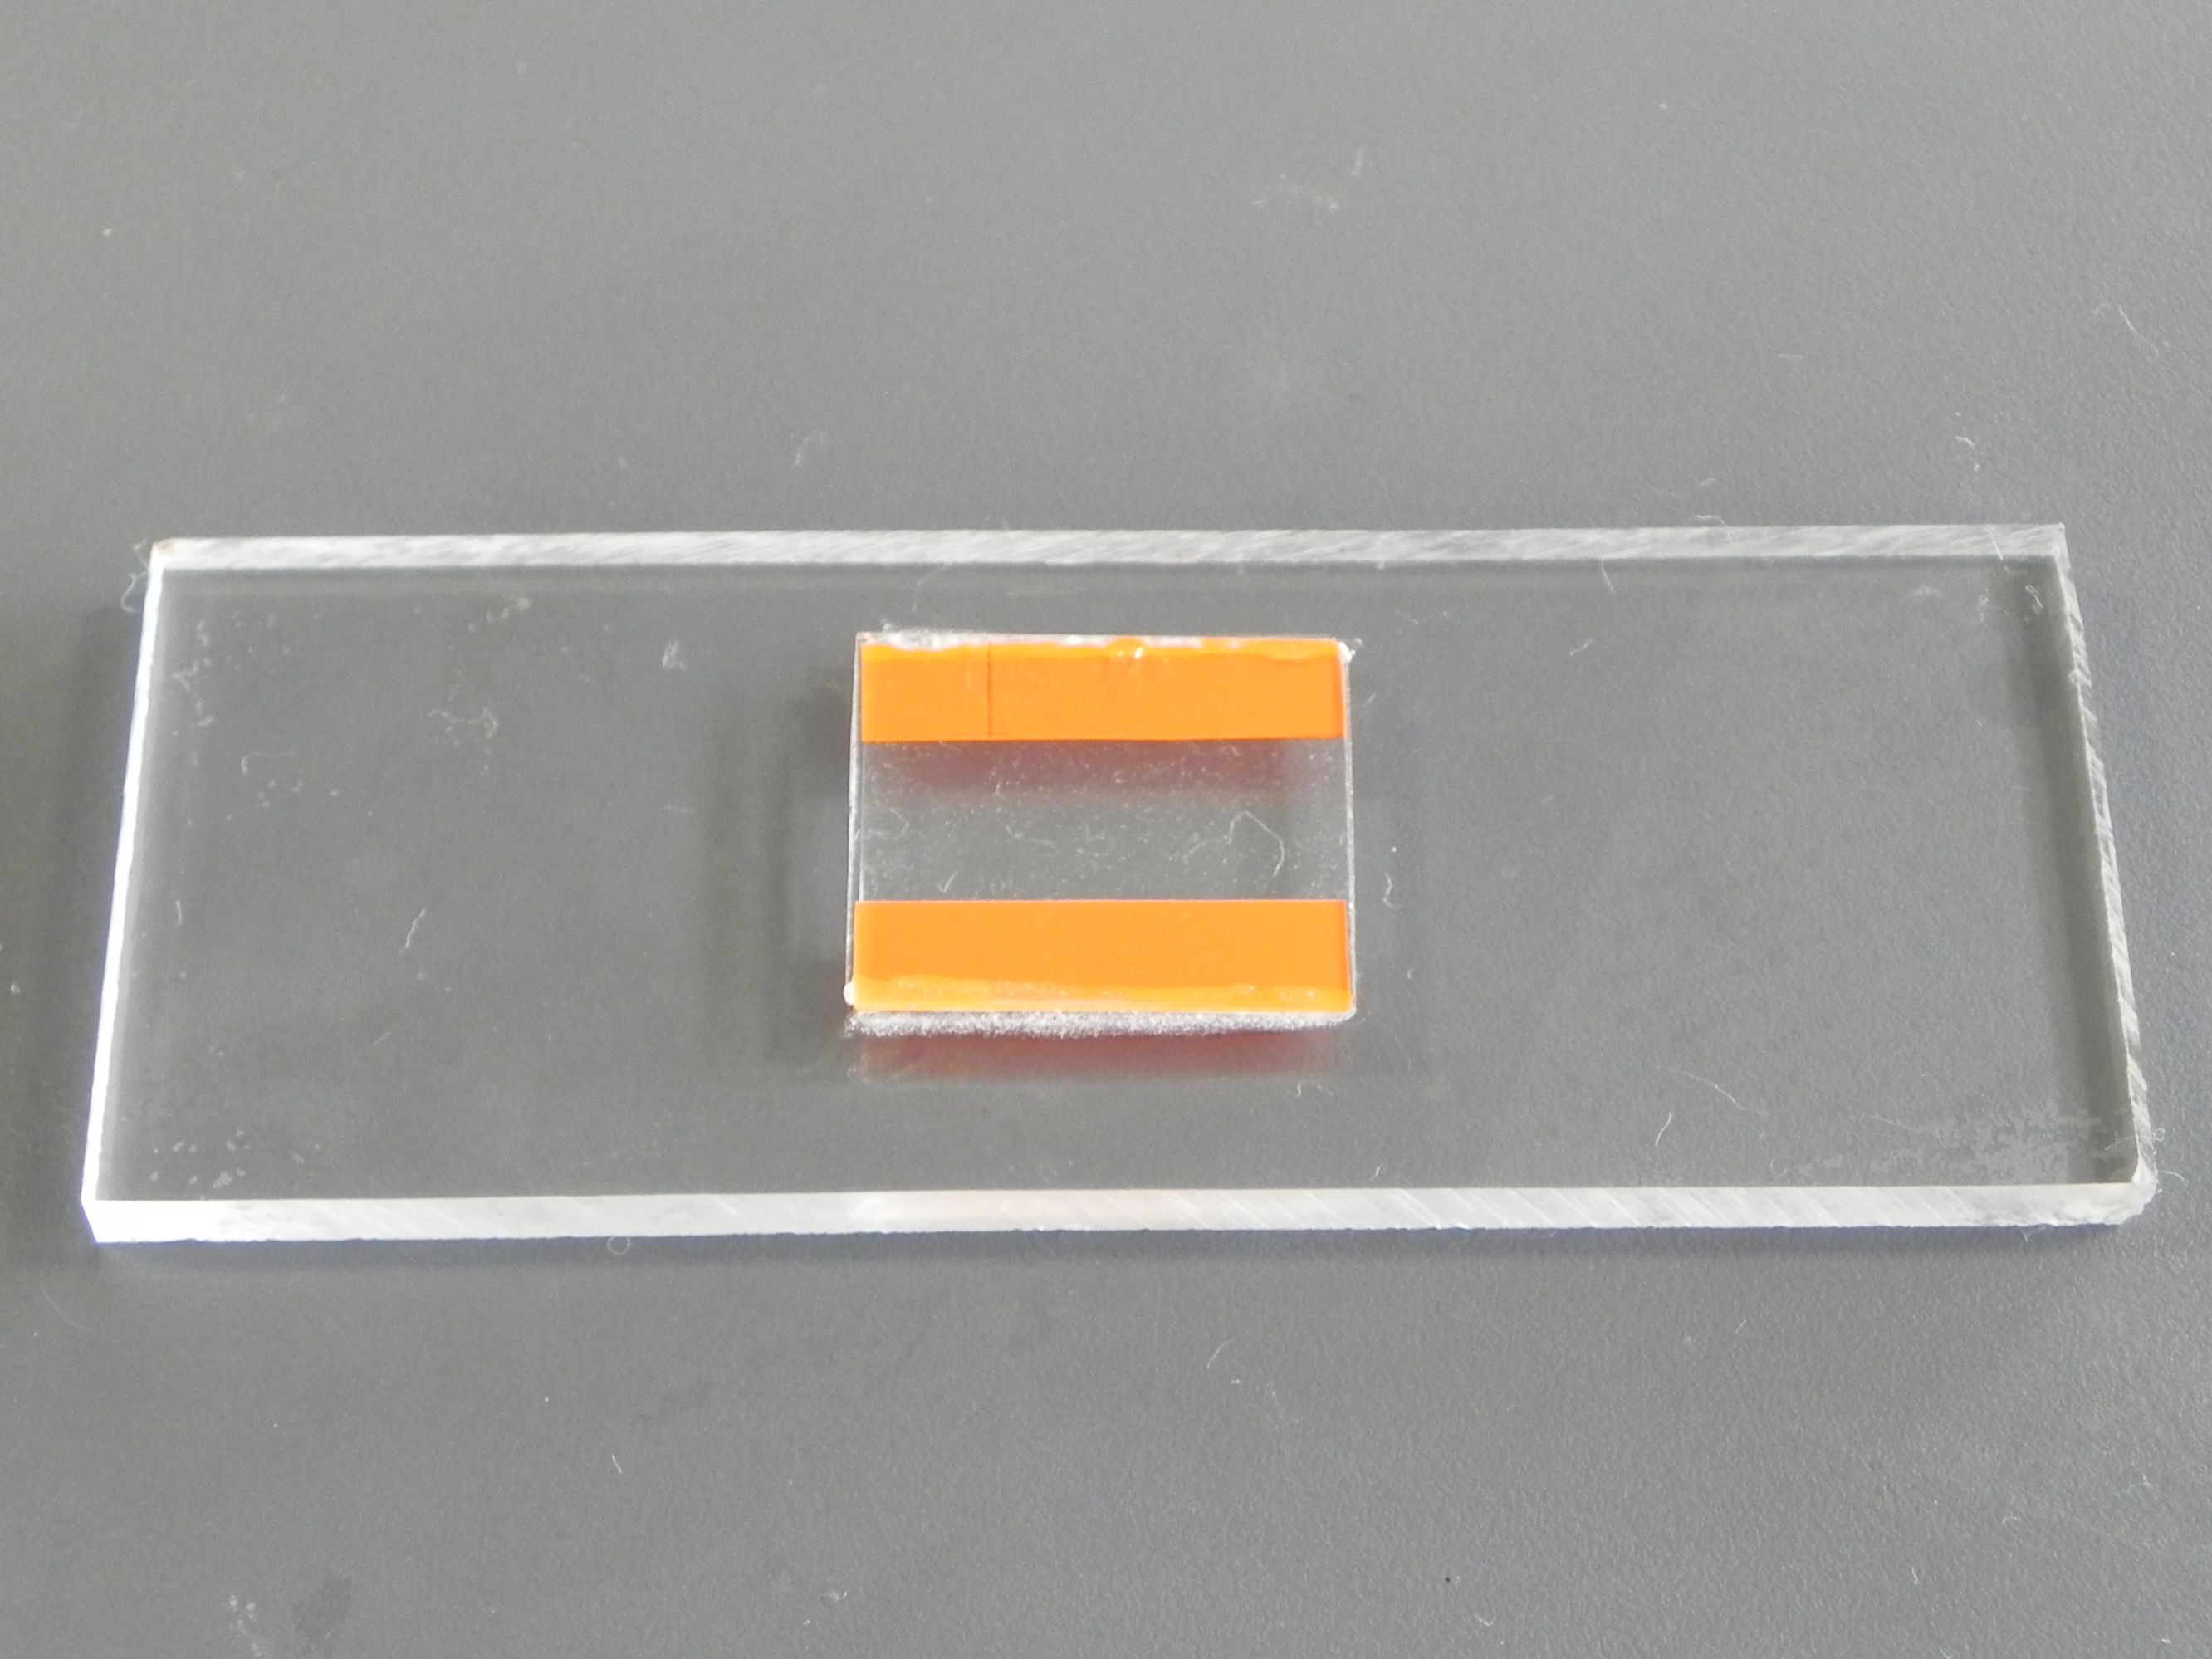
\includegraphics[width=0.5\textwidth]{content/pt1/01-PowerHarvesting/graphics/Photo_streamingPotential_Assembly_Step2.JPG}
        \par\end{centering}

\centering{}\protect\caption{\label{Photo_streamingPotential_Assembly_Step2}Photo
    showing shims sandwiched between two slide halves} \end{figure}
\begin{figure}[p] \begin{centering}
        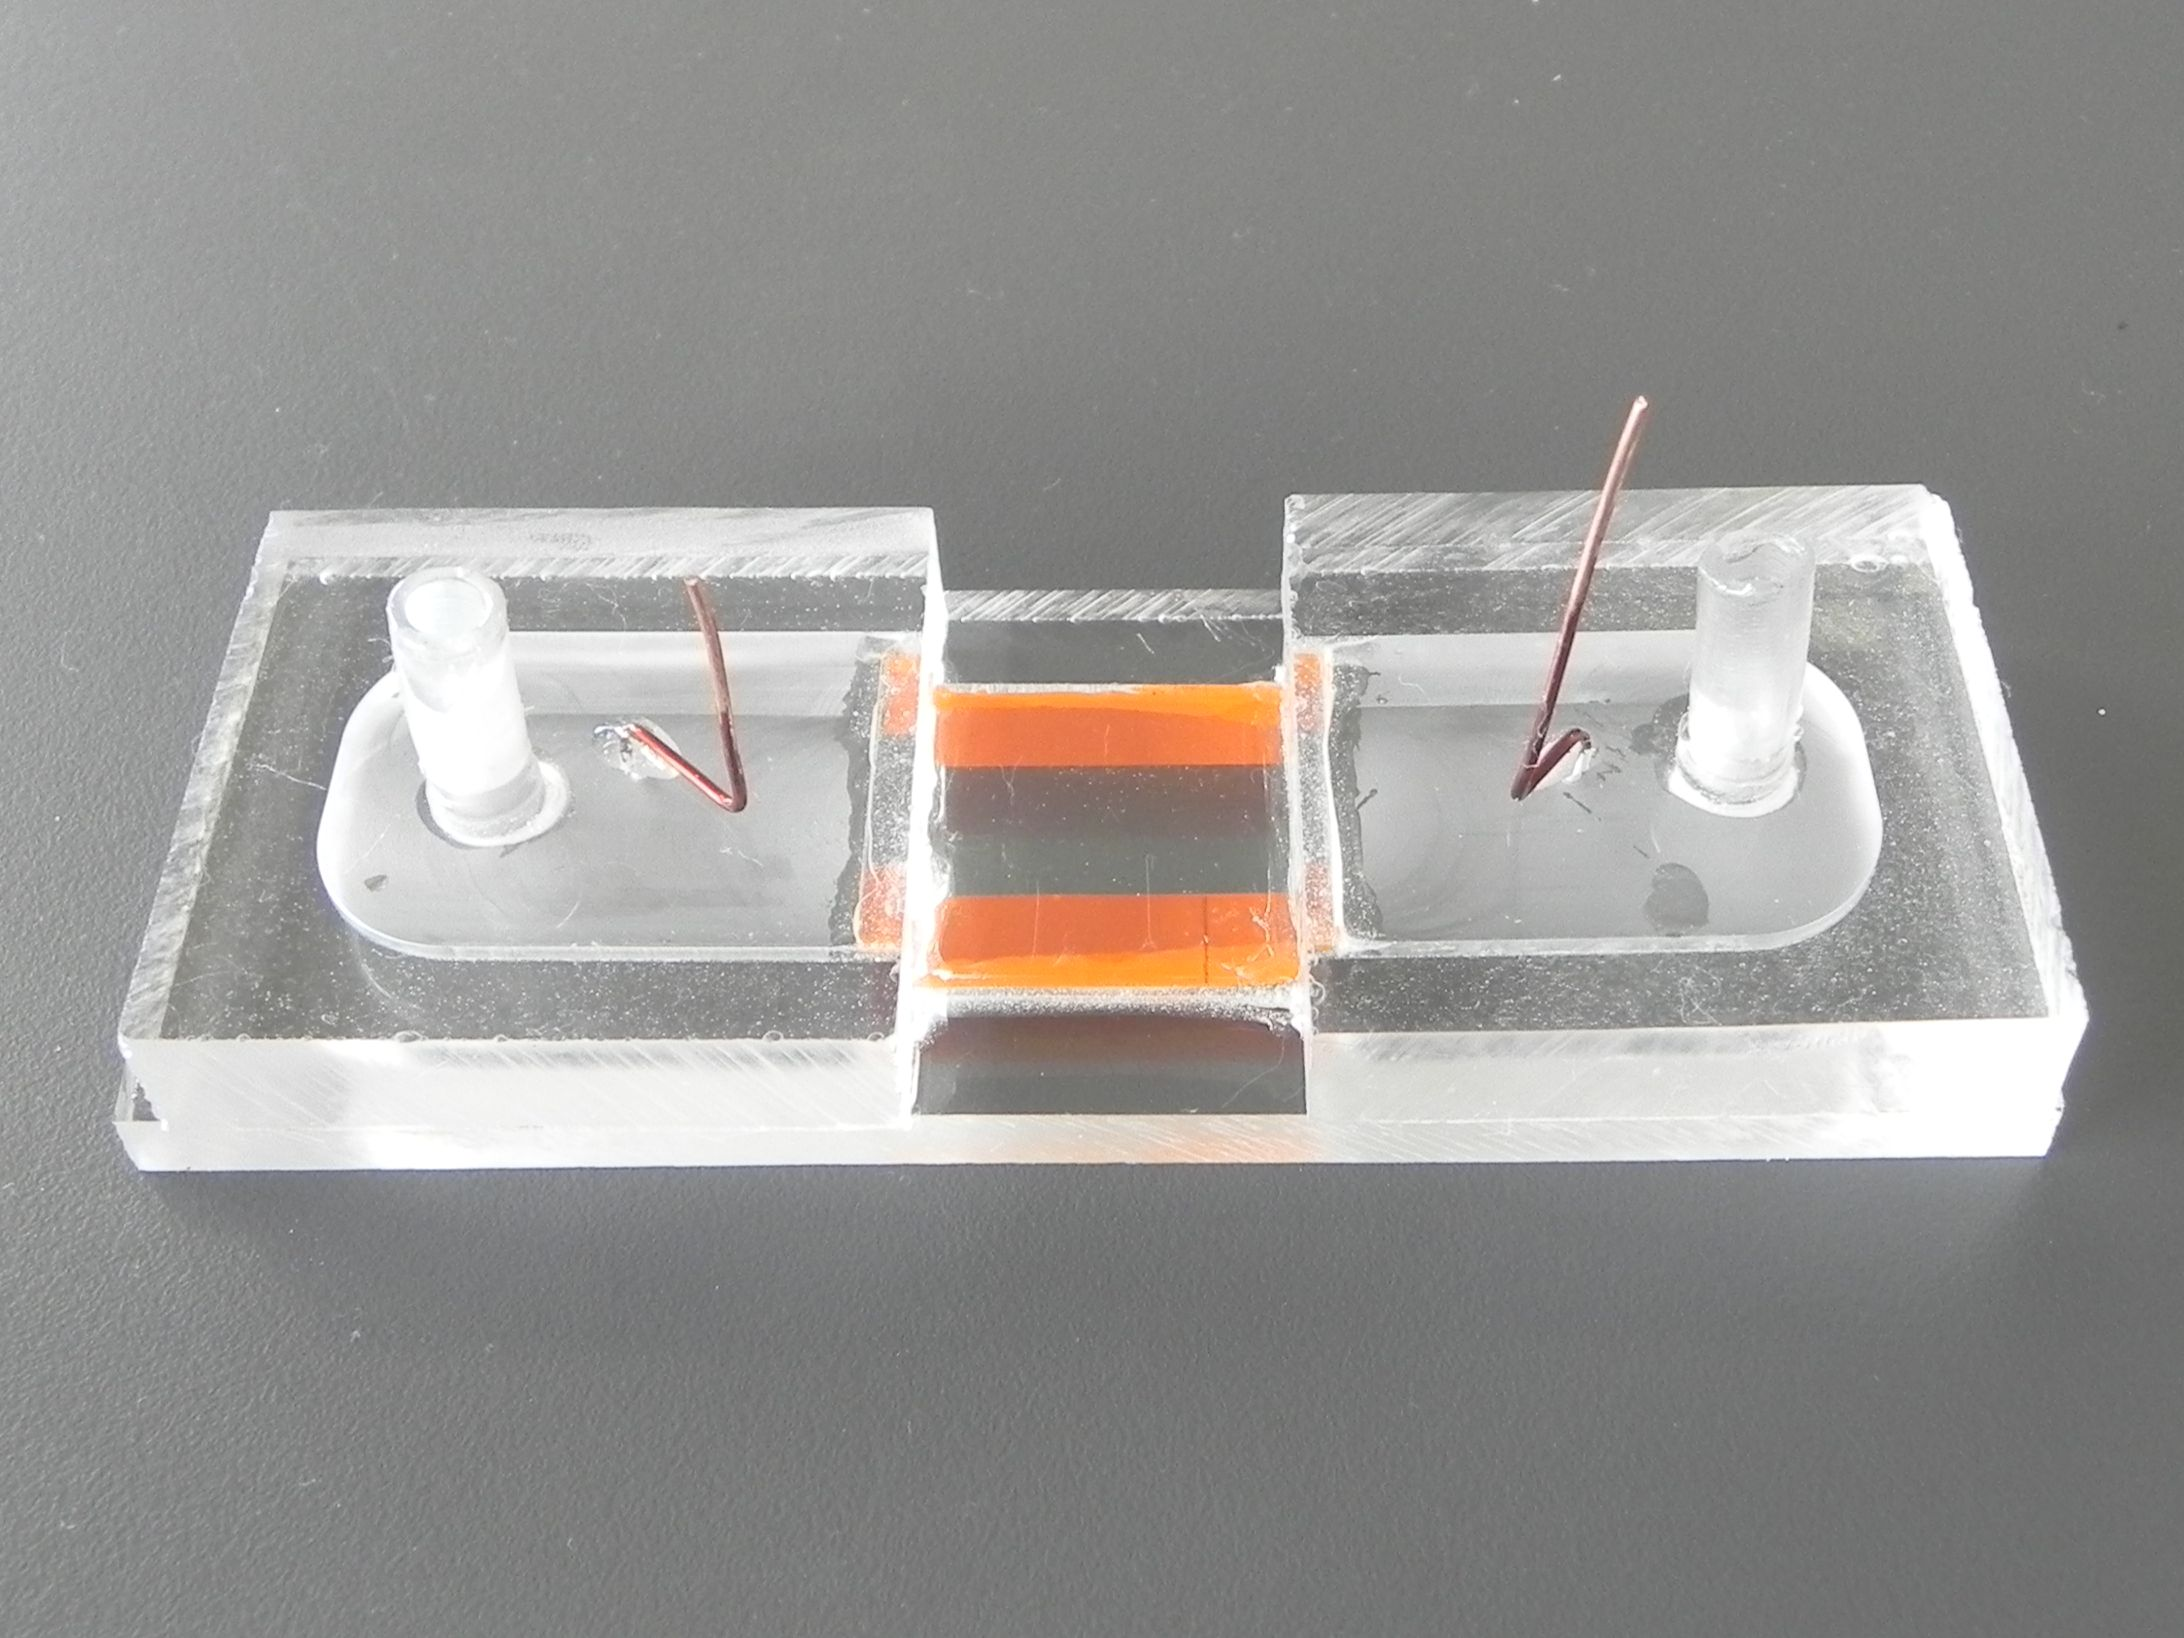
\includegraphics[width=0.5\textwidth]{content/pt1/01-PowerHarvesting/graphics/Photo_streamingPotential_Assembly_Step3.JPG}
        \par\end{centering}

\centering{}\protect\caption{\label{Photo_streamingPotential_Assembly_Step3}Photo
    showing final assembly} \end{figure} \begin{figure}
\begin{tabular}{|c|c|c|} \hline Microscope slides & Sail Brand & JIA 7101WT -
    26 x 76mm\tabularnewline \hline Shims & Garlock & Colorplast - 50$\,\mu$m,
    80$\,\mu$m, 120$\,\mu$m and 250$\,\mu$m\tabularnewline \hline Epoxy &
    Selleys & Araldite - Ultra Clear Resin\tabularnewline \hline Pressure
    Sensor & Honeywell & 24PC15SMT - 0 -- $\pm$15 PSI\tabularnewline \hline
\end{tabular}

\protect\caption{\label{Table_StreamingCell_MaterialsUsed}Table of materials
    used to construct the streaming potential cells} \end{figure}


First, glass microscope slides where cut in half to give panels of glass that
where approximately 26 x 38mm. Once such glass panel can be seen in Figure
\ref{Photo_streamingPotential_Assembly_Step1}.  Next, two pieces of shim
material where placed on either side of the glass panel with a small amount of
epoxy, on top of which another glass panel was placed. Pressure was applied to
the panels pressing them together while the epoxy set to create the channel
that can be seen in Figure \ref{Photo_streamingPotential_Assembly_Step2}. Each
channel was photographed under microscope once set to determine the height of
the channel created. Finally, acrylic couplers where mounted over each end,
again by the use of epoxy. These couplers allowed the water to be forced
through the channel while providing mounting for the voltage sensing wires. The
final assembly is shown in Figure
\ref{Photo_streamingPotential_Assembly_Step3}.


\subsubsection*{Measurement}

Each assembly was connected between the tap and drain of a lab basin.  To
facilitate measurement of the pressure gradient across the channel, a pressure
transducer was placed across the input and output ports of the channel
assembly. Single core copper wire was used to measure voltage gradients across
the channel. These wires where epoxied into the couplers to reduce leaks. To
conduct the measurements an Agilent E5270B Precision Measurement Mainframe was
used, which has an input impedance of 10${\displaystyle \, T\Omega}$. The high
input impedance of this machine ensures that the measurements are not disturbed
by current leaking through the measurement device. The E5270 was responsible
for measuring the output of the pressure transducer and the voltage across the
channel.


\subsection{Results}

Ten cavities ranging in height from 26$\,\mu m$ to 245$\,\mu m$ where built and
measured. Individual plots showing pressure applied versus voltage developed
are shown in Appendix \ref{sec:Appendix-Streaming-Potential-Cell}.  For
convenience, a graph with the steepest voltage per pressure gradient is shown
in Figure \ref{fig:streamingCell_voltVsPress_52um_convienient}, which resulted
from using a cell with a height of 52$\,\mu m$.

\begin{figure}[H] \centering
    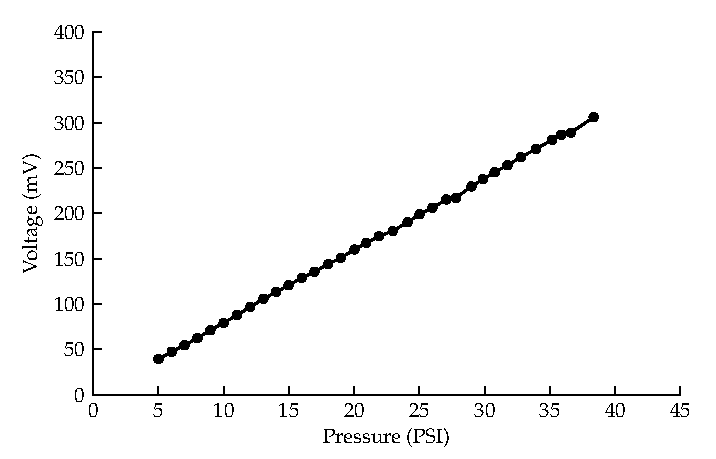
\includegraphics{content/pt1/01-PowerHarvesting/graphics/streamingCell_voltVsPress_52um_out}
    \caption{\label{fig:streamingCell_voltVsPress_52um_convienient}Line graph
        showing voltage output versus pressure for a 52$\,\mu m$ glass
        micro-channel.} \end{figure}


From the results obtained it is clear that there is a definite \nobreakdash-
linear \nobreakdash- relationship between the amount of pressure applied and
the voltage developed across each channel. Figure
\ref{fig:streamingCell_scatter_voltGradVsHeight} compares the gradient of
voltage developed per PSI of pressure for each of the channels. The graph shows
a trend toward larger voltage development as channel height is reduced to
around 50$\,\mu m$. Below 50$\,\mu m$ it is unclear what to expect from the
channel which will require further investigation. Spread in the data is
expected to be the result of epoxy (used to glue the slides together) seeping
into the cavity, thereby slightly altering each cavity's dimensions.

\begin{figure} \begin{centering}
        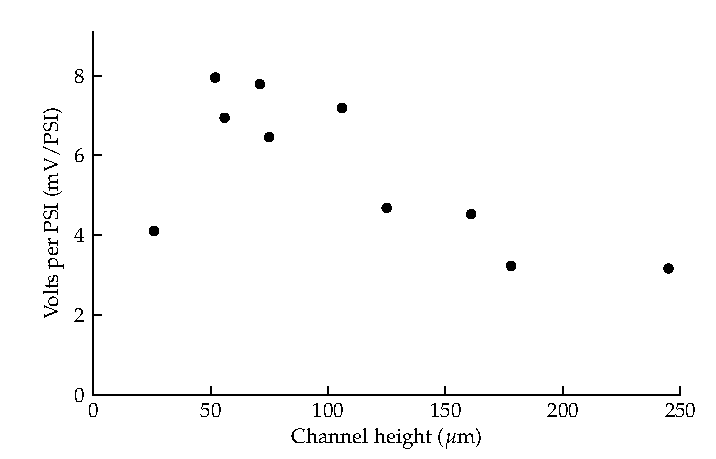
\includegraphics{content/pt1/01-PowerHarvesting/graphics/streamingCell_slopeVsChannelHeight}
        \par\end{centering}

\protect\caption{\label{fig:streamingCell_scatter_voltGradVsHeight}Scatter plot
    of voltage/pressure gradient versus channel height for each of the measured
    channels.}


\end{figure}



\subsection{Conclusion}

Power generation from streaming potential cells is possible, this is evident
from the voltages developed in this experiment. The streaming cell is capable
of producing output when operated using standard tap water at standard tap
pressures. As yet, the amount of current that can be drawn from such a channel
has not been ascertained, and therefore the amount of available power remains
unknown (although it is estimated to be in the very small). An initial estimate
of the ideal channel lies between 25-75$\,\mu m$ in height.


\section{Governing Model}


\subsection{Charge separation analysis}

As mentioned at the beginning of this chapter, for a streaming potential cell
to operate there must be an electrical potential at the interface between solid
and liquid matter. In the experiment that Wayne Crump and myself replicated,
the solid/liquid interface was between glass and standard Hamilton tap water,
so where does this electrical potential come from?

Quoting Tandon et al. in \cite{Tandon2008}: Many microfluidic substrates behave
as weak acids in aqueous solutions. In glass substrates, surface silanol groups
can be deprotonated in aqueous solutions leaving a negative surface charge:

\begin{equation}
    SiOH\overset{^{K_{a}}}{\mathbf{\rightleftharpoons}}SiO^{-}+H^{+}
\end{equation}


It is this deprotonation that is responsible for generating the charge
difference at the glass/liquid surface of the microchannel and therefore
establishing an electrical double layer (EDL). Since the charge imbalance in
this case arises from the fact that the glass behaves as a weak acid, the
process itself is affected by the pH of the liquid, something we have no
control over when using tap water.

Once an ionic double layer within the channel has been established, ``the
streaming potential is engendered by the flow of the ions relative to the
stationary charged wall of the channel'' \cite{Mansouri2005}.  This flow is
accomplished in our case by applying a pressure gradient across the channel.
``The ratio of streaming potential to pressure gradient depends on the zeta
potential''\cite{Park2009}


\subsection{\label{sub:StreamingCell-Mathematics}Mathematics}

The first step toward optimisation is to define all the parameters that
describe the device. The streaming current, which is defined as the electrical
current that flows in the direction of water flow, is defined in
\cite{Olthuis2005} to be:

\begin{equation} I_{s}=\frac{A\,\varepsilon_{0\,}\varepsilon_{r}}{\eta\,
        l}\Delta P\,\zeta\label{eq:StreamingCell_StreamingCurrentFunc}
\end{equation} where: \begin{description} \item [{$\varepsilon_{0}$}] is the
        permittivity of free space \item [{$\varepsilon_{r}$}] is the relative
        permittivity of the liquid \item [{$\eta$}] is the viscosity of the
        liquid \item [{$l$}] is the length of the channel \item [{$\Delta P$}]
        is the pressure difference across the channel \item [{$\zeta$}] is the
        zeta-potential of the of the glass-liquid interface \item [{$A$}] is
        the cross-sectional area of the channel, or combined area of multiple
        channels \end{description} This equation indicates that the cell will
produce a current that is proportional to the amount of pressure across it and
that the output is affected by the geometry of the channel itself. To help
model the situation it is convenient to break Equation
\ref{eq:StreamingCell_StreamingCurrentFunc} formula down in the following
manner: \begin{eqnarray} I_{s} & = & \Delta P\,\left(\frac{A}{\eta\,
            l}\right)\,\left(\varepsilon_{0}\,\varepsilon_{r}\,\zeta\right)\nonumber
    \\ I_{s} & = & \frac{\Delta P}{\left(\frac{\eta\,
                l}{A}\right)}\,\left(\varepsilon_{0}\,\varepsilon_{r}\,\zeta\right)\nonumber
    \\ I_{s} & = & \frac{\Delta
        P}{R_{h}}\,\left(\varepsilon_{0}\,\varepsilon_{r}\,\zeta\right)\label{eq:StreamingCurrent_HydrostaticResistance}\\
    \frac{I_{s}}{\Delta P} & = &
    \frac{\varepsilon_{0}\,\varepsilon_{r}\,\zeta}{R_{h}}\nonumber \\ g_{m} & =
    & \frac{\varepsilon_{0}\,\varepsilon_{r}\,\zeta}{R_{h}}\nonumber
\end{eqnarray}


where $R_{h}$ is the hydrodynamic resistance caused by the channel, $g_{m}$
represents the transconductance between pressure applied and current produced
and $I_{s}$ is the streaming current. The hydrodynamic resistance ($R_{h}$)
will be affected by the geometry of the channel so $R_{h}$ is considered an
approximation of the hydrodynamic resistance.

Once the cell begins to separate charge a current in the reverse direction is
established called the conduction current ($I_{c}$).

Ohms law states:

\[ I=\frac{V}{R} \]


In this situation the resistance is determined by the conductivity of the water
($\sigma$), as well as the cross sectional area ($A$) and length ($l$) of the
channel.

\[ R=\frac{l}{\sigma\, A} \]


Therefore, the conduction current back through the channel is determined by:

\begin{equation} I_{c}=A\sigma\frac{V_{s}}{l} \end{equation}


Where $\sigma$ is the conductivity of the liquid and $V_{s}$ is the voltage
developed across the channel. This is also shown in

At equlibrium the streaming current ($I_{s}$) and the conduction current
($I_{c}$) are equal and opposite in direction.


\subsection{\label{sub:Electrical-model}Electrical model}

Figure \ref{fig:StreamingCell_Schematic-representation} depicts schematically
how a streaming cell would operate when connected to an external load.  This
model is based upon that found in \cite{Olthuis2005} by Olthuis et al. but has
been modified to show the pressure applied ($\Delta P$) as the voltage source,
instead of the zeta potential ($\zeta$). It is the pressure that responsible
for creating the streaming current; a zeta potential on its own simply isn't
enough. This has been shown through the results obtained in Appendix
\ref{sec:Appendix-Streaming-Potential-Cell}, where $V_{s}$ was directly
proportional to $\Delta P$; as $V_{s}$ is directly related to $I_{s}$ as per
Ohm's law.

\begin{figure} \begin{centering}
        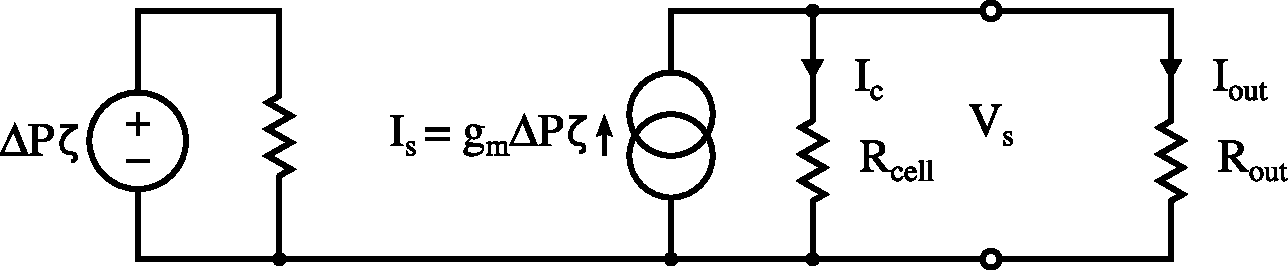
\includegraphics[scale=0.55]{content/pt1/01-PowerHarvesting/graphics/StreamingCell_EquivalentCircuit_output}
        \par\end{centering}

\protect\caption{\label{fig:StreamingCell_Schematic-representation}Schematic
    representation of a streaming cell with attached output resistance}
\end{figure}



\subsection{Output analysis}

The electrical model described in \ref{sub:Electrical-model} shows how the cell
would operate with a load placed across the cell. By combining this model with
the equations from \ref{sub:StreamingCell-Mathematics} it should be possible to
see the effect that altering various cell parameters has on the output.

\begin{eqnarray} P & = & V\times I\nonumber \\ V & = & I\times R\nonumber \\ P
    & = & I^{2}\times R\nonumber \\ P_{out} & = & I_{out}^{2}\times
    R_{out}\nonumber \\ I_{out} & = &
    I_{s}\times\frac{R_{cell}}{R_{cell}+R_{out}}\nonumber \\ P_{out} & = &
    \left[I_{s}\times\frac{R_{cell}}{R_{cell}+R_{out}}\right]^{2}\times
    R_{out}\label{eq:DeterminingOutputPower} \end{eqnarray}



\subsubsection*{Finding an optimum value for $R_{out}$}

Using Ohm's Law it is possible to find an equation that give the output power
as a function of the electrical resistance of the cell ($R_{cell)}$) and the
output resistance ($R_{out}$) as shown in Equation
\ref{eq:DeterminingOutputPower}.  In order to optimise the output power it is
necessary to find the value of output resistance ($R_{out}$) that maximises the
output power.

Next I take Equation \ref{eq:DeterminingOutputPower} and treat the streaming
current ($I_{s}$) as a constant, differentiate with respect to $R_{out}$ and
find the condition that gives a maximum/minimum power output.

\begin{eqnarray*} \frac{\partial P_{out}}{\partial R_{out}} & = &
    \frac{R_{cell}^{2}}{(R_{cell}+R_{out})^{2}}-\frac{2\times
        R_{cell}^{2}\times R_{out}}{(R_{cell}+R_{out})^{3}}\\ 0 & = &
    \frac{R_{cell}^{2}}{(R_{cell}+R_{out})^{2}}-\frac{2\times
        R_{cell}^{2}\times R_{out}}{(R_{cell}+R_{out})^{3}}\\ \frac{2\times
        R_{cell}^{2}\times R_{out}}{(R_{cell}+R_{out})^{3}} & = &
    \frac{R_{cell}^{2}}{(R_{cell}+R_{out})^{2}}\\ \frac{2\times
        R_{cell}^{2}\times R_{out}}{R_{cell}+R_{out}} & = & R_{cell}^{2}\\
    2\times R_{cell}^{2}\times R_{out} & = &
    R_{cell}^{2}\times(R_{cell}+R_{out})\\ 2\times R_{out} & = &
    R_{cell}+R_{out}\\ R_{out} & = & R_{cell} \end{eqnarray*}


This shows that there is either maximum or minimum power transfer to $R_{out}$
when the value of $R_{out}$ matches that of $R_{cell}$, which is shown to be a
maximum as per Figure \ref{fig:Plot-of-PowerThereom}.  This result is
consistant with that of the Maximum Power Thereom, which I had trouble finding
a reference of for a current source and resistances in parallel. It shows that
in order to achieve the maximum possible output power, that the load should
have a resistance equal to that of the electrical resistance of the cell
itself. Additionally, it was found that the absolute magnitudes of both
$R_{out}$ and $R_{cell}$ have no effect on the output power, so long as they
are equal to one another.

\begin{figure}
    \begin{centering}
        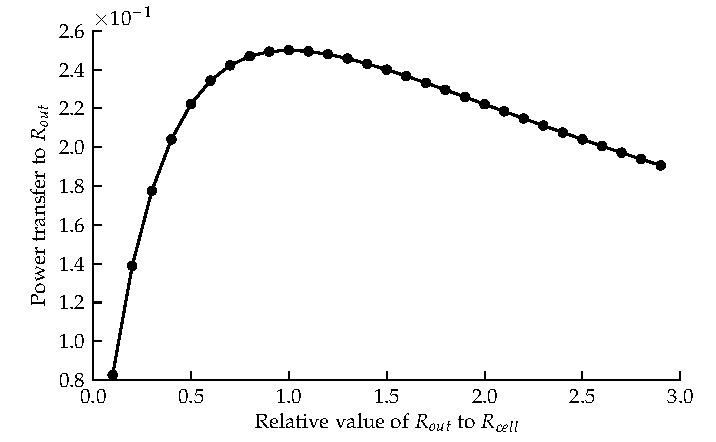
\includegraphics{content/pt1/01-PowerHarvesting/graphics/maximumPowerThereom}
        % 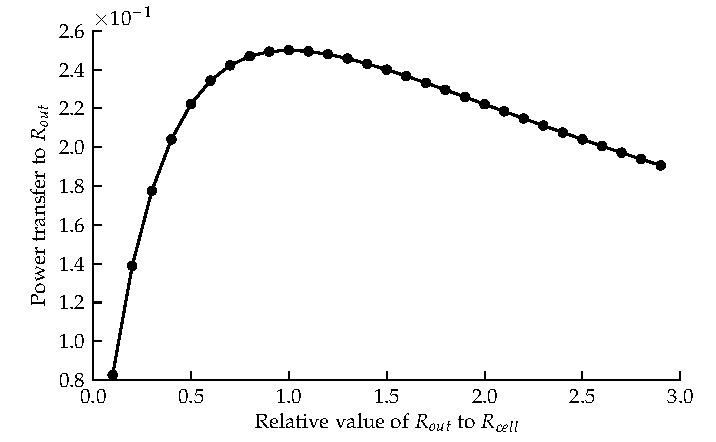
\includegraphics{content/pt1/01-PowerHarvesting/graphics/maximumPowerThereom}
    \end{centering}
    \caption{\label{fig:Plot-of-PowerThereom}Plot of Equation \ref{eq:DeterminingOutputPower} when $I_{s}=1A$ and $R_{cell}=1\Omega$}
\end{figure}


This can now be used to calculate the maximum available power as a function of
$I_{s}$ by substituting $R_{out}$ and $R_{cell}$ for $R$ , as
$R_{out}=R_{cell}=R$:

\begin{eqnarray} P_{out} & = &
    \left[I_{s}\times\frac{R_{cell}}{R_{cell}+R_{out}}\right]^{2}\times
    R_{out}\nonumber \\ P_{max} & = &
    \left[I_{s}\times\frac{1}{2}\right]^{2}\times R\nonumber \\ P_{max} & = &
    \frac{I_{s}^{2}R}{2}\label{eq:streamingCell_maxPower} \end{eqnarray}


And as $P=I^{2}R$ (via the power equation and Ohm's Law) this indicates that at
most we can hope to havest half of the total power, while the other half is
dissipated back through $R_{cell}$. Combining Equations
\ref{eq:streamingCell_maxPower} and
\ref{eq:StreamingCurrent_HydrostaticResistance} gives:

\begin{eqnarray*} P_{max} & = & \frac{\left(\frac{\Delta
                P}{R_{h}}\,\left(\varepsilon_{0}\,\varepsilon_{r}\,\zeta\right)\right)^{2}R}{2}\\
    P_{max} & = & \frac{\left(\frac{\Delta
                P\,\varepsilon\,\zeta}{R_{h}}\right)^{2}R}{2}\\ P_{max} & = &
    \frac{\Delta P^{2}\,\varepsilon^{2}\,\zeta^{2}R}{2R_{h}^{2}}
\end{eqnarray*}


where $\varepsilon=\varepsilon_{0}\,\varepsilon_{r}$ and $R=R_{cell}=R_{out}$ .
If we now substitute $R$ and $R_{h}$ for their respective functions we end up
with:

\begin{eqnarray} P_{max} & = & \frac{\Delta
        P^{2}\,\varepsilon^{2}\,\zeta^{2}R}{2R_{h}^{2}}\nonumber \\ P_{max} & =
    & \frac{\Delta P^{2}\,\varepsilon^{2}\,\zeta^{2}\,\left(\frac{l}{\sigma\,
                A}\right)}{2\left(\frac{\eta\, l}{A}\right)_{h}^{2}}\nonumber
    \\ P_{max} & = & \frac{\Delta P^{2}\,\varepsilon^{2}\,\zeta^{2}\,
        l}{\sigma\, A}\times\frac{1}{\frac{2\eta^{2}\, l^{2}}{A^{2}}}\nonumber
    \\ P_{max} & = & \frac{\Delta P^{2}\,\varepsilon^{2}\,\zeta^{2}\, l\,
        A^{2}}{\sigma\, A\,2\eta^{2}\, l^{2}}\nonumber \\ P_{max} & = &
    \frac{\Delta P^{2}\,\varepsilon^{2}\,\zeta^{2}\, A}{2\,\sigma\,\eta^{2}\,
        l}\nonumber \\ P_{max} & \propto & \frac{\Delta P^{2}\,\zeta^{2}\,
        A}{l}\nonumber \\ P_{max} & \propto & \frac{\Delta
        P^{2}\,\zeta^{2}}{R_{h}} \end{eqnarray}



\subsubsection*{Optimisation of $R_{h}$ and $\Delta P$}

Knowing the optimum value of output resitance leaves only the streaming current
($I_{s}$) and it's constituants as optimisation parameters.  Equation
\ref{eq:StreamingCurrent_HydrostaticResistance} indicates that in order to
further optimise the cell, one must reduce hydrodynamic resistance ($R_{h}$)
and increase both the Zeta potential ($\xi$) and pressure difference ($\Delta
P$) placed across the cell.

We can model the water supply, harvester and a consumer as a basic electrical
circuit as shown in Figure \ref{fig:Schematic-model-of-harvester}.  In this
model $P_{supply}$ represents the total water pressure available, Flow
represents the flow rate of water, $R_{h}$ and $R_{consumer}$ are the
hydrodynamic resistances of the harvesting cell and a water consumer (e.g. a
house) respecively and $\Delta P$ is the pressure developed difference across
the harvester, where $R_{h}\propto\frac{l}{A}$.

\begin{figure} \begin{centering}
        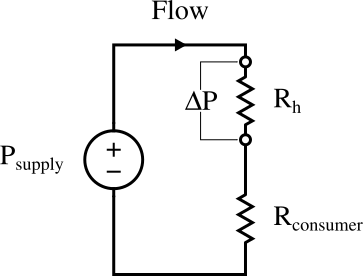
\includegraphics[scale=0.55]{content/pt1/01-PowerHarvesting/graphics/Harvester_equivalentCircuit_output}
        \par\end{centering}

\protect\caption{\label{fig:Schematic-model-of-harvester}Schematic model of the
    water supply, harvester and consumer}


\end{figure}


\begin{figure} \begin{centering}
        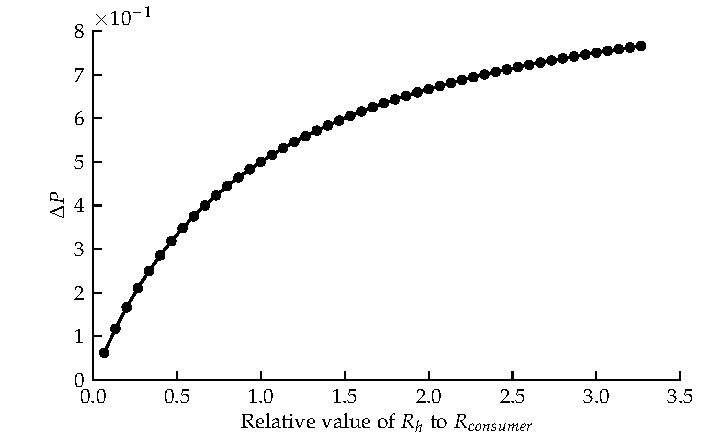
\includegraphics{content/pt1/01-PowerHarvesting/graphics/streamingCell_consumerModel_dP}
        \par\end{centering}

\protect\caption{\label{fig:Effect-of-varying-Rh-onP}Effect of varying $R_{h}$
    on $\Delta P$ for the harvester/consumer model shown in Figure
    \ref{fig:Schematic-model-of-harvester}.}


\end{figure}


\begin{figure} \begin{centering}
        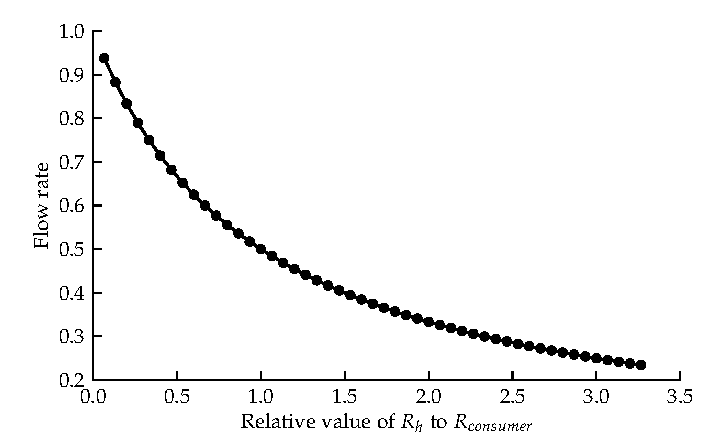
\includegraphics{content/pt1/01-PowerHarvesting/graphics/streamingCell_consumerModel_flow}
        \par\end{centering}

\protect\caption{\label{fig:Effect-of-varying-Rh-onFlow}Effect of varying
    $R_{h}$ on Flow for the harvester/consumer model shown in Figure
    \ref{fig:Schematic-model-of-harvester}.} \end{figure}


\begin{figure} \begin{centering}
        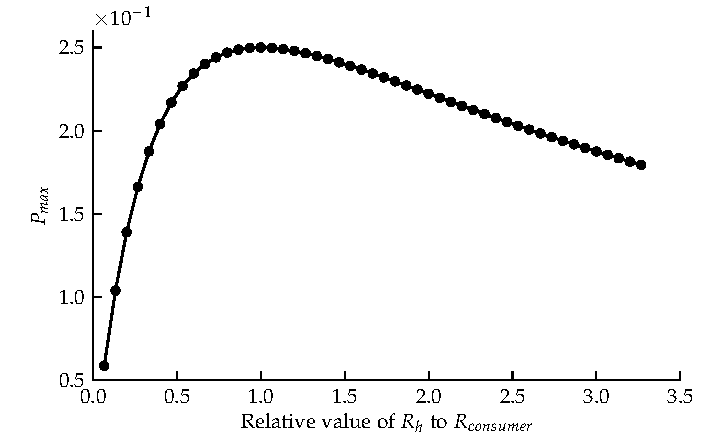
\includegraphics{content/pt1/01-PowerHarvesting/graphics/streamingCell_consumerModel_total}
        \par\end{centering}

\protect\caption{\label{fig:Effect-of-varying-Rh-onIs}Effect of varying $R_{h}$
    on \foreignlanguage{english}{$P_{max}$} for the harvester/consumer model
    shown in Figure \ref{fig:Schematic-model-of-harvester}.} \end{figure}
Figures \ref{fig:Effect-of-varying-Rh-onP},
\ref{fig:Effect-of-varying-Rh-onFlow} and \ref{fig:Effect-of-varying-Rh-onIs}
show how varying $R_{h}$ will affect $\Delta P$, the flow rate and the value of
$\frac{\Delta P}{R_{h}}$ respectively. Notice in Figure
\ref{fig:Effect-of-varying-Rh-onP} that increasing $R_{h}$ has the effect of
increasing $\Delta P$.  Optimisation wise, the benifit of increasing $I_{s}$ by
increasing $\Delta P$ is opposed by also increasing the value of $R_{h}$
(referring to Equation \ref{eq:StreamingCurrent_HydrostaticResistance}).

Figure \ref{fig:Effect-of-varying-Rh-onFlow} shows how the value of $R_{h}$
affects the flow rate through the system. Keeping the flow rate high is
important in order to ensure that the consumer does not notice a drop in water
pressure due to the addition of the harvester in their water system.

Finally, Figure \ref{fig:Effect-of-varying-Rh-onIs} shows the effect that
varying $R_{h}$ has on \foreignlanguage{english}{$P_{max}$} (according to
$P_{max}\propto\frac{\Delta P^{2}\,\zeta^{2}}{R_{h}}$ when $\zeta=1$). The
result is the same as that of Equation \ref{eq:DeterminingOutputPower}, showing
that this is again goverend by the maximum power transfer thereom. Practically,
a harvester that dropped half of the supply pressure would not be feasable in
most domestic situations, so a trade-off will have to be made that meets
plumbing standards.


\subsubsection*{Optimisation of the Zeta potential}

Referring back to Equation \ref{eq:StreamingCell_StreamingCurrentFunc}, I have
determined how to increase the total output of the harvester by choosing
appropriate values for all of the parameters except $\varepsilon_{r}$ and
$\zeta$. As the harvester will be using domestic tap water the value of
$\varepsilon_{r}$ will be that of the relative permittivity of water, and is
therefore relatively fixed (being only affected by the temperature of the
water). This leaves $\zeta$ as the remaining parameter.



\chapter{Applicability to Water Metering}
  \label{chap:wirelessWaterMetering}
  \section{Current Trends in Water Metering}
  \section{Appropriatenes of Streaming Cell Harvesters}

  A method of power harvesting was put forward in chapter \ref{chap:harvestingEnergy} that used water flow as a source of energy.
  We expect the lack moving parts in that design will reduce or eliminate maintenance costs.
  Such a low maintenance harvester is ideal for water utility companies to measure and record water usage.
  This chapter discusses how such a water meter might be implemented.
  The content in this chapter is used as the basis for investigating the energy requirements of such a harvester.
  
\section{Power Consumption}

\begin{figure}
\begin{centering}
\protect\caption{Power consumption of ZigBee}

\par\end{centering}

\end{figure}
\begin{figure}

\begin{centering}
\protect\caption{Power consumption of RFM12B}

\par\end{centering}

\end{figure}



\chapter{Energy Requirements}
  \label{chap:energyRequirements}
  
  \section{Microcontrollers}
      %!TEX root = ../../../thesis.tex

Harvesting power directly from flowing water opens the possibility of low-maintenance smart metering.


At the heart of a smart metering system is the microcontroller (MCU),
which among other things will be keeping track of the amount of water
consumed. In order to know whether it is possible to extract enough
power from a domestic water supply it is necessary to assess how much
power is required to run a microprocessor and any associated hardware.

In this chapter I compare power consumption and operational efficiencies
of six low power MCUs deemed suitable for running a power harvesting
water meter. The microprocessors to be investigated are low power,
general purpose 8-bit MCUs from three mainstream manufacturers, Microchip,
Atmel and Freescale. Measurement of power consumption will be carried
out during processing, sleeping and whilst undertaking two tasks that
are essential for smart water metering, analog-to-digital conversion
and non-volatile writes to memory.


\section{Selection}

The following microprocessors have been chosen as they represent a
well spaced selection from the three mainstream MCU manufacturers.
\begin{itemize}
\item Microchip PIC16F1827
\item Microchip PIC16F688
\item Microchip PIC12F675
\item Atmel ATtiny25V
\item Atmel ATtiny13V
\item Freescale MC9S08QG8
\end{itemize}
A basic feature comparison of the MCU selection is shown in table
%\ref{tab:MCUfeaturecomparison}.

\begin{sidewaystable}
\begin{centering}
\begin{tabular}{|l|l|l|l|l|l|l|l|}
\cline{2-8}
\multicolumn{1}{l|}{} & PIC16F1827  & PIC16F887  & PIC16F688  & PIC12F675  & ATtiny25V  & ATtiny13V  & MC9S08QG8 \tabularnewline
\hline
Vdd (min)  & 1.8  & 2.0  & 2.0V  & 2.0  & 1.8  & 1.8  & 1.8 \tabularnewline
Vdd (max)  & 5.5  & 5.5  & 5.5V  & 5.5  & 5.5  & 5.5  & 3.6 \tabularnewline
I (sleep)  & 30nA  & 50nA  & 50nA  & 1nA  & 100nA & <100nA & 450nA\tabularnewline
CLOCK (min)  & 31kHz  & 31kHz & 31kHz & 31kHz & 16kHz & 16kHz & 1MHz \tabularnewline
CLOCK (max)  & 32MHz  & 8MHz  & 8MHz  & 4MHz  & 16MHz & 9MHz  & 10MHz\tabularnewline
EEPROM  & 256B  & 256B  & 256B  & 128B  & 128B  & 64B  & \dag{}\tabularnewline
Serial  & USI  & USI  & USI  & --  & USI  & --  & USI \tabularnewline
USART  & UART  & UART  & UART  & --  & --  & --  & -- \tabularnewline
ADC  & 10bit  & 10bit & 10it  & 10bit & 10bit & 10bit & 10bit\tabularnewline
\hline
\end{tabular}
\par\end{centering}

\begin{centering}
\dag Has 8,192 bytes of software programmable flash (16 pages of 512
bytes each).
\par\end{centering}

\begin{centering}
\ddag Has 256 bytes of software programmable flash (4 pages of 64
bytes each).
\par\end{centering}

\centering{}\protect\caption{\label{tab:MCUfeaturecomparison} Feature comparison of selected MCUs.}
\end{sidewaystable}



\section{Power consumption}

Each of the MCUs were programmed to carry out various tasks which
were performed over their specified range of operating voltages and
operating frequencies. While the chips where carrying out these tasks
their power consumption was measured by an Agilent E5270B Precision
Mainframe via a PC and a Tektronix MSO 4054 Oscilloscope for timing
purposes. Details on how each of the tests where carried out, as well
as raw data, can be found in appendix %\ref{Appendix:Measurements} .


\subsection{Test conditions}

Where possible the chips were configured to have each of their pins
set to outputs, held high, whilst being tied to Vdd via 10k$\Omega$
resistors. All chips had their peripherals disabled (where appropriate)
including any watchdog timers and brownout detection circuitry.

To allow more accurate sleep current measurements, the chips were
placed in a chip carrier with 10k$\Omega$ resistors soldered between
the pins (except ground and Vdd) and Vdd. They chip and carrier was
then washed in isopropyl alcohol and dried before being suspended
by connections to the the E5270. These steps were taken to reduce
any current leakage between pins due to fingerprints or dirt.


\subsection{Sleeping}

\begin{figure}
\begin{centering}
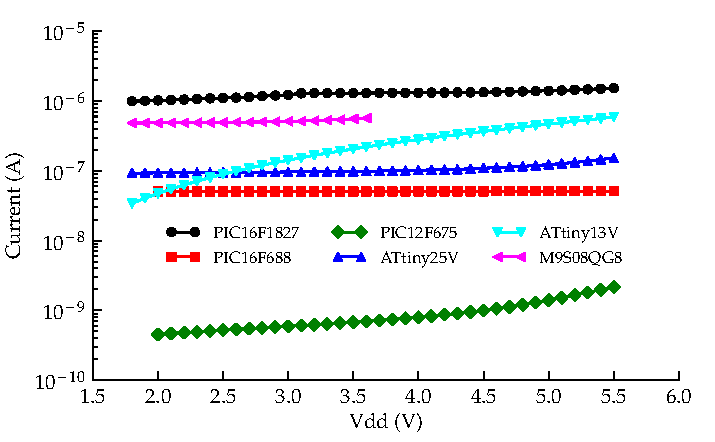
\includegraphics{content/pt1/02-Microcontrollers/graphics/Graph_All_Sleeping_Current}
\par\end{centering}

\centering{}\protect\caption{\label{fig:All_Sleep_Current}Current consumed by investigated MCUs
while in sleep mode.}
\end{figure}


A microprocessor in sleep mode is basically switched off, the only
difference being that volatile data is preserved provided the input
voltage doesn't fall below a minimum threshold voltage. In order to
consume as little power as possible an MCU should spend as much time
in sleep mode as is feasible. Power consumption during sleep therefore
plays a significant role in a chips ability to conserve power over
time.

\prettyref{fig:All_Sleep_Current} shows the amount of current consumed
by each of the MCUs while in their sleep state, note the log scale
on the y-axis. It can be seen that the PIC16F1827 consumes the most
current. This is somewhat contradictory to its specified sleep current
of 30nA \cite{PIC16F1827} (the second lowest of the set) at almost
1000 times higher. The Freescale MC9S08QG8 consumed energy at an average
of 11\% higher than specified \cite{MC9S08QG8}. Both the Atmel ATtiny13V
and ATtiny25V fell within their specification, \cite{AtmelATtiny13}
and \cite{AtmelATtiny25} respectively. There appears to be a trade-off
made between the two chips in the way of minimum power consumption
and minimum response to Vdd. The ATtiny13V required approximately
2.7 times less power than the ATtiny25V at 1.8V, but this advantage
rapidly falls away as Vdd moves up from 1.8V (and negated after 2.5V
Vdd). The Microchip PIC12F675 fell within specification\cite{PIC12F675}
and was the clear winner of the tested MCUs.

As the PIC16F1827 was so far off its specified value, the measurement
was repeated numerous times using code written in both assembler and
HI-TECH C as well as trying five different chips. All steps in the
datasheet to reduce power consumption where followed and all configuration
options where set, however no improvement was made.


\subsection{Processing}

Measuring the amount of power it takes to process information is not
a simple task. The way each chip carries out processing operations
internally can be quite different from one another, even though they
all produce the same result. This section will focus on the the energy
consumed while processing data and executing code.


\subsubsection{Behind the scenes \label{sub:Behind-the-scenes}}

\begin{table}
\begin{centering}
\begin{tabular}{|c|c|}
\cline{2-2}
\multicolumn{1}{c|}{} & Instructions\tabularnewline
\hline
PIC16F1827 & 53\tabularnewline
\hline
PIC16F688 & 35\tabularnewline
\hline
PIC12F675 & 35\tabularnewline
\hline
ATtiny25V & 120\tabularnewline
\hline
ATtiny13V & 120\tabularnewline
\hline
MC9S08QG8 & 145\tabularnewline
\hline
\end{tabular}
\par\end{centering}

\centering{}\protect\caption{\label{tab:Number-of-instructions}Instruction set size for each tested
MCU.}
\end{table}


Not all MCUs are created equal, however this doesn't mean that some
are simply ``better'' than others. There are many complex factors
that determine the suitability of a particular MCU for a specific
task, one of which is the ability to crunch numbers. This section
is intended to give some background in plain-english of the relevant
inner workings that affect computational performance.

\begin{algorithm}[H]
\begin{lstlisting}
if (danger >= 5) flight();
else flee();
\end{lstlisting}
\protect\caption{\label{alg:Simple-C-code-representation}Simple C-code representation
of a branch instruction.}
\end{algorithm}


Algorithm \ref{alg:Simple-C-code-representation} shows a simplified
portion of C-code to demonstrate (very simply) how it may be implemented
in various ways. To determine whether or not the outcome of the code
is to fight or flee, the processor must first evaluate whether or
not the variable `danger' is greater than or equal to five and either
branch to the function `flight' or continue on to execute the function
`flee'.

\begin{algorithm}
\begin{lstlisting}
load 5 into register 001
load danger into register 002
branch-if-greater-or-equal 001 002 flee_call
call-subroutine fight
jump-to continue
[flee_call]
call-subroutine flee
[continue]
\end{lstlisting}
\protect\caption{\label{alg:Psudo-machine-code1}Psudo machine-code representation
of a branch instruction.}
\end{algorithm}





\begin{algorithm}
\begin{lstlisting}
load danger into register 001
subtract-from-register 001 5
branch-if-minus 001 fight_call
call-subroutine flee
jump-to continue
[fight_call]
call-subroutine fight
[continue]
\end{lstlisting}
\caption{\label{alg:Psudo-machine-code2}Psudo machine-code representation
of an alternative branch instruction.}
\end{algorithm}


Algorithms \ref{alg:Psudo-machine-code1} and \ref{alg:Psudo-machine-code2}
demonstrate two slightly different ways of implementing \ref{alg:Simple-C-code-representation}
in pseudo machine-code. The decision of which is best is made by the
compiler, which should take the instructional efficiency of the specific
MCU into account. This is an overly simplistic example, but its main
point is to illustrate that there are multiple paths that lead to
the same result. The important thing to note is that not all of those
paths require the same amount of effort. This means that the compiler's
ability to optimise code efficiently plays a role in determining the
overall performance of the chip. This also means that the programmer
shouldn't need to worry too much about instructional efficiency as
the compiler should transform C-code into machine code that best suits
the target MCU.

Another factor in processing efficiency comes down to the number of
different things (or instructions) it can do. All instructions for
each MCU are defined in its instruction set. Most 8-bit MCUs are based
on reduced instruction set computing (RISC) architecture, as opposed
to complex instruction set computing (CISC). This means that when
compared CISC based CPU, a RISC based chip is simpler and therefore
usually cheaper to produce. ``Instruction traces from CISC machines
consistently show that few of the available instructions are used
in most computing environments''\cite{ComputerArch}, meaning that
a lot of the added complexity in CISC designs is mostly underutilised.
To prevent confusion, a processor with a small instruction set can
perform all the same calculations that a processor with a larger instruction
set can so they are no less capable in a calculation sense. What this
means is that the processor with the reduced instruction set may need
to execute multiple instructions in order to achieve the same result
as an instruction from another processor which it doesn't have.

The final thing to note when comparing performance is that the clock
frequency of an MCU isn't necessarily the frequency at which it performs
operations, although sometimes it is.


\subsubsection{Power consumed while processing}

\begin{figure}
\begin{centering}
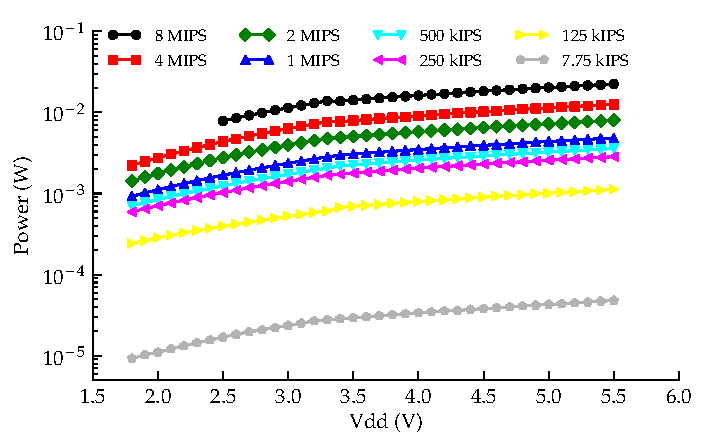
\includegraphics{content/pt1/02-Microcontrollers/graphics/Graph_PIC16F1827_Clock_Power}
\par\end{centering}

\protect\caption{\label{graph:CLK_POWER_16F1827}Power consumed by the PIC16F1827 while
processing}
\end{figure}
\begin{figure}
\begin{centering}
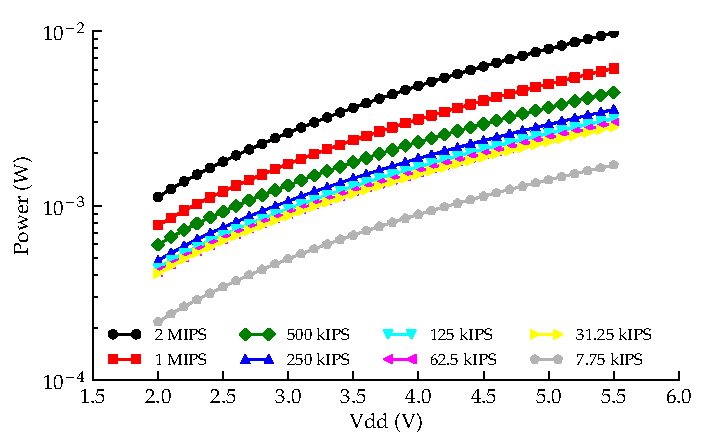
\includegraphics{content/pt1/02-Microcontrollers/graphics/Graph_PIC16F688_Clock_Power}
\par\end{centering}

\protect\caption{\label{graph:CLK_POWER_16F688}Power consumed by the PIC16F688 while
processing}
\end{figure}
\begin{figure}
\begin{centering}
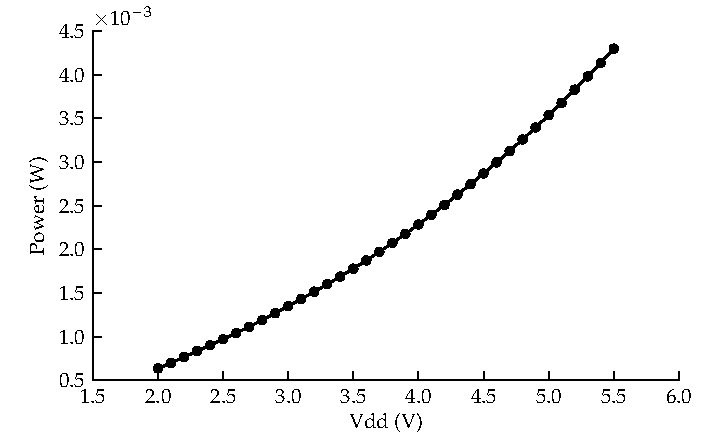
\includegraphics{content/pt1/02-Microcontrollers/graphics/Graph_PIC12F675_Clock_Power}
\par\end{centering}

\protect\caption{\label{graph:CLK_POWER_12F675-1}Power consumed by the PIC12F675 while
processing}
\end{figure}
\begin{figure}
\begin{centering}
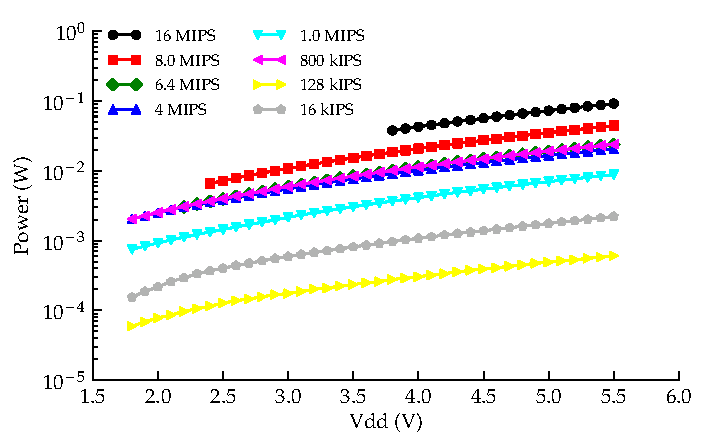
\includegraphics{content/pt1/02-Microcontrollers/graphics/Graph_ATtiny25V_Clock_Power}
\par\end{centering}

\protect\caption{\label{graph:CLK_POWER_ATtiny25V}Power consumed by the ATtiny25V
while processing}
\end{figure}
\begin{figure}
\begin{centering}
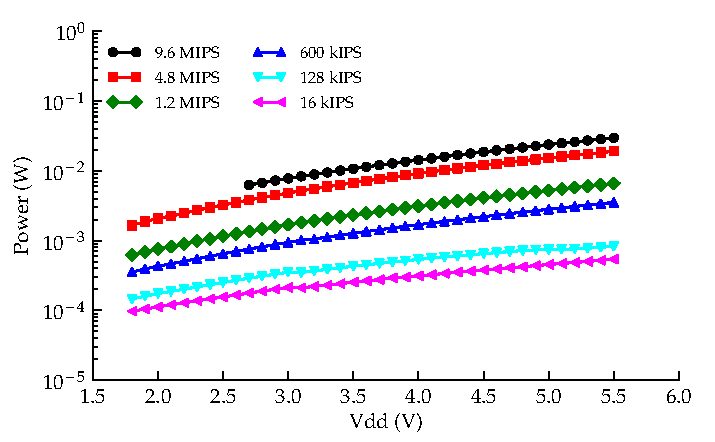
\includegraphics{content/pt1/02-Microcontrollers/graphics/Graph_ATtiny13V_Clock_Power}
\par\end{centering}

\protect\caption{\label{graph:CLK_POWER_ATtiny13V}Power consumed by the ATtiny13V
while processing}
\end{figure}
\begin{figure}
\begin{centering}
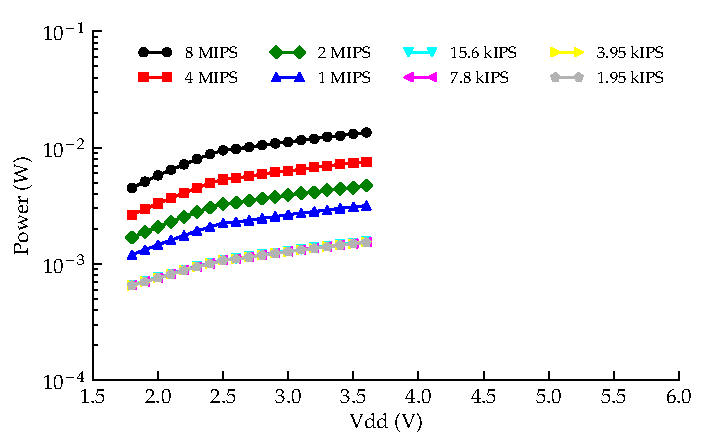
\includegraphics{content/pt1/02-Microcontrollers/graphics/Graph_MC9S08QG8_Clock_Power}
\par\end{centering}

\protect\caption{\label{graph:CLK_POWER_MC9S08QG8}Power consumed by the MC9S08QG8
while processing}
\end{figure}


The Microchip PIC16F1827 displayed the lowest energy usage with 10$\mu A$
while clocking 7.75kIPS (as shown in figure \ref{graph:CLK_POWER_16F1827}).
It should be noted that the Microchip MCUs complete one instruction
cycle for every four clock cycles, so the 7.75kIPS corresponds to
a clock frequency of 31kHz. Also, not all instructions take one instruction
cycle to complete (as discussed in section \ref{sub:Behind-the-scenes}).
Figure \ref{graph:CLK_POWER_16F688} shows that the PIC16F688 consumes
less power than the PIC16F1827 while at low voltages for the same
instruction rates (except at 7.75kIPS). However, there appears to
be a flatter response in power consumption with respect to Vdd in
the PIC16F1827, similar to what was seen in figure \ref{fig:All_Sleep_Current}
with the Atmel chips.The PIC12F675 (as shown in \ref{graph:CLK_POWER_16F688})
used the same at the PIC16F688 (figure \ref{graph:CLK_POWER_16F688})
for its 1MIPS trace. Figures \ref{graph:CLK_POWER_ATtiny25V} and
\ref{graph:CLK_POWER_ATtiny13V} show both Atmel MCUs having similar
power requirements.The MC9S08QG8, although being able to clock the
slowest, performed very poorly at low frequencies. At 1.95kIPS it
consumed approximately the same amount of power as the Microchip MCUs
operating at 1MIPS.


\subsubsection{Joules of energy consumed per instruction cycle\label{sub:Joules-of-energy}}

A convenient, and more insightful way to interpret the previous processing
power consumption graphs is to calculate the energy spent per instruction
performed. The energy cost of an instruction cycle can be calculated
using equation \ref{eq:JPI calculation}.

\begin{equation}
J_{i}=\frac{I\times Vdd}{f_{i}}\label{eq:JPI calculation}
\end{equation}
where $J_{i}$ is the number of joules consumed per instruction, $I$
is the current draw, $Vdd$ is the input voltage and $f_{i}$ is the
instruction frequency.

Figure \ref{fig:Per-instruction-cycle} compares the most energy efficient
operating conditions of each of the tested chips. What is most interesting
about this graph is amount of overlap between each of the chips. Also,
these greater efficiencies occur at high operating frequencies. A
simple rule of thumb for selecting the most power efficient operating
frequency based on these results is to choose the highest frequency
where the MCU can operate over its full input voltage (Vdd) range.
For comparison, figure \ref{fig:Per-instruction-ATtiny13V} shows
the trade-off made when selecting a higher frequency, which is typical
across the range of MCUs tested.

\begin{figure}
\begin{centering}
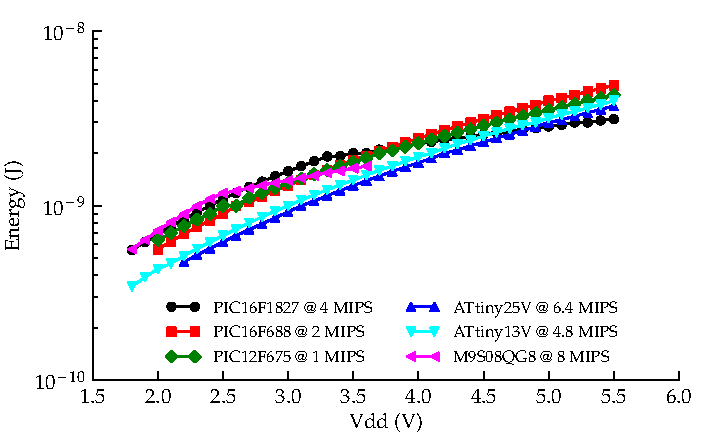
\includegraphics{content/pt1/02-Microcontrollers/graphics/Graph_All_Clock_JPI}
\par\end{centering}

\protect\caption{\label{fig:Per-instruction-cycle}Per instruction cycle energy consumption
comparison}
\end{figure}
\begin{figure}
\begin{centering}
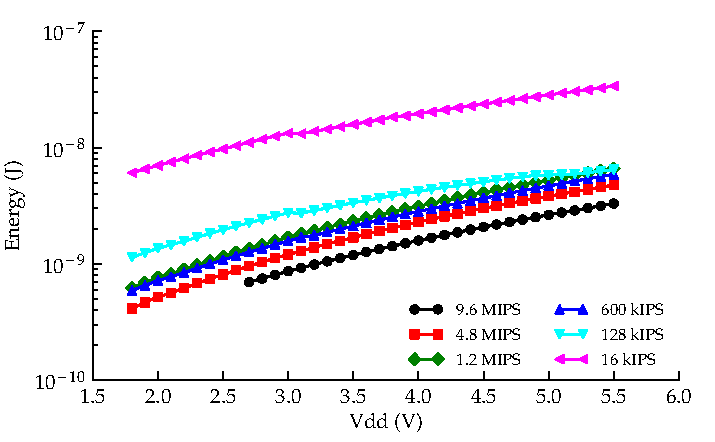
\includegraphics{content/pt1/02-Microcontrollers/graphics/Graph_ATtiny13V_Clock_JPI}
\par\end{centering}

\protect\caption{\label{fig:Per-instruction-ATtiny13V}Per instruction cycle energy
consumption of the ATtiny13V}
\end{figure}



\subsubsection{Performance benchmark}

In section \ref{sub:Joules-of-energy} I presented a graph showing
the amount of energy consumed per instruction cycle for each MCU under
ideal operating conditions. But, as discussed in section \ref{sub:Behind-the-scenes},
not all instructions take one instruction cycle to complete. Also,
some MCUs have extra instructions that are designed to help speed-up
code execution by combining commonly used pairs of instructions. This
section will look at how many instruction cycles each MCU takes to
complete a benchmarking function. Which will allow a more accurate
representation of execution efficiency to be made.

For the benchmarking function I wanted something that would consume
a large number of instructions cycles, be well suited to an 8-bit
microcontroller (i.g. no complex maths functions and small memory
footprint) and have a well defined end point. For this I chose a linear
feedback shift register based pseudo-random number generator (as shown
in \ref{alg:Benchmarking-algorithm}), for which the code was sourced
from \cite{LinearFeedbackRegister}.

In short, this function starts with a 16-bit number and runs it through
the linear feedback register in a tight loop until the initial value
of the 16-bit feedback register is produced again. This function steps
through every possible combination of bits possible in a 16-bit number
(except zero; 65535) in a pseudo-random order before exiting the loop.
The function combines the exclusive-OR (XOR), bit shifting, bitwise
AND, increment a value and numerical comparison operations in a tight
loop.

\begin{algorithm}
\begin{lstlisting}
unsigned short lfsr = 0xACE1u;
unsigned period = 0;
do {
	lfsr = (lfsr >> 1) ^ (-(lfsr & 1u) & 0xB400u);
	++period;
} while(lfsr != 0xACE1u);
\end{lstlisting}
\caption{\label{alg:Benchmarking-algorithm}Benchmarking algorithm}
\end{algorithm}


The benchmarking function was compiled and run on each of the MCUs
operating at a range of frequencies. The amount of time each MCU took
to complete the benchmark was timed by watching a pin that toggled
on completion of the benchmark function with a Tektronix MSO 4054
Oscilloscope. The number of instruction cycles each chip took to complete
the benchmark was deduced by multiplying the time taken to complete
the benchmark by the instruction cycle frequency. The results of the
benchmark are shown in figure \ref{fig:GraphBar_All_Benchmark}. It
should be noted that to calculate the number of instruction cycles
taken by the Microchip family of processors (PIC16F1827, PIC16F688
and PIC12F675) the chip frequency divided by four was used, meaning
that the number of clock cycles consumed was four times higher. It
is clear from figure \ref{fig:GraphBar_All_Benchmark} that the Atmel
(ATtiny25V and ATtiny13V) microprocessors are by far the most efficient
microprocessor in terms of executing code using a minimum number of
instructions of the selection.

\begin{figure}
    \begin{centering}
        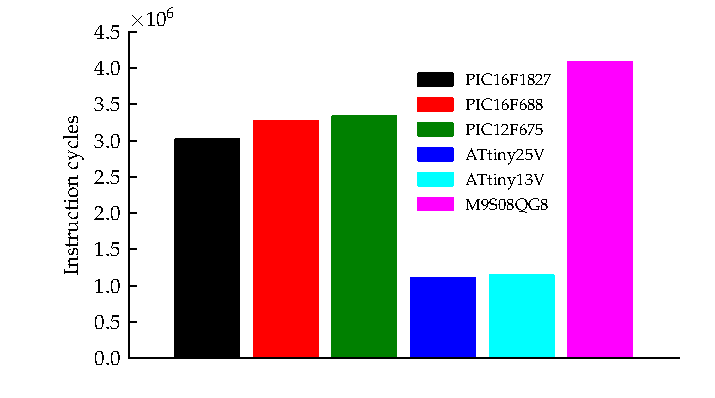
\includegraphics{content/pt1/02-Microcontrollers/graphics/Graph_All_Clock_Benchmark}
    \end{centering}
    \protect\caption{\label{fig:GraphBar_All_Benchmark}MCU comparison of instructions
    taken to complete a benchmark.}
\end{figure}



\subsection{Non-volatile memory}

In order for a microprocessor to keep information about its current
state and recorded data in the event of power loss it must write to
non-volatile memory. Non-volatile memory is implemented as either
electrically erasable and programmable read only memory (EEPROM) or
Flash memory. Flash memory is similar to EEPROM with the exception
that it must be erased in large blocks, or pages, before it can be
written to. All of the tested MCUs have on-board EEPROM with the exception
of the MC9S08QG8 which has flash memory instead. Table \ref{tab:MCUfeaturecomparison}
shows the amount of non-volatile memory space available on each of
the chips. The energy consumption of each of the chips with EEPROM
memory during a 1-byte write operation (which also includes a 1-byte
erase operation) is shown in figure \ref{fig:Energy-consumed-EEPROM}.
There appears to be a glitch with the PIC12F675 with respect to it's
energy consumption. It's energy consumption was calculated as negative
with a Vdd below 4.7V, meaning that it consumed less current while
performing write operations than running through the same program
loop without performing writes. The measurement was repeated several
times and produced the same result but I did not further pursue the
cause. I have concluded that this is not representative of the MCU
and have disregarded EEPROM measurement data for this chip. In the
case of the MC9S08QG8, which has Flash memory instead of EEPROM, the
power consumption in the E + W case was calculated per erase/write
operation to be $1/512^{th}$ of the page erase energy consumption
added to the energy cost of a single write operation, where the W
case was the energy cost of a single write operation. In order for
the MC9S08QG8 to perform a write operation, the destination byte must
have already been pre-erased at an earlier point in time. This may
be useful for power harvesting since the energy expensive page erase
operation, which consumes an average of 3.02e-4 Joules, can be done
performed when available energy is plentiful.

\begin{figure}
\begin{centering}
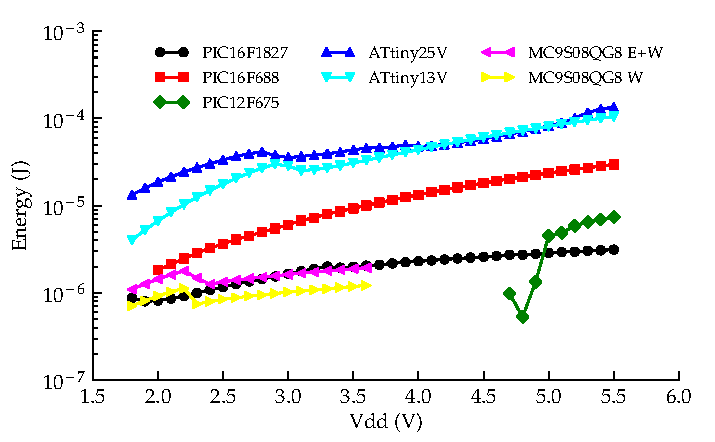
\includegraphics{content/pt1/02-Microcontrollers/graphics/Graph_All_EEPROM_JPO}
\par\end{centering}

\protect\caption{Energy consumed by each MCU per non-volatile erase/write operation.\label{fig:Energy-consumed-EEPROM}}
\end{figure}



\subsection{Analog-to-digital conversions.}

To measure the flow of water the chosen MCU will likely either count
pulses record a voltage level from a flow meter. It is possible that
another mechanism such as ultrasonic flow measurement may be used
but for now only analog-to-digital (ADC) measurements will be measured.
For those unfamiliar with an ADC, it is simply a way of converting
a voltage (which is generally free to change) into a digital number
that a MCU can process and/or store. The power consumption per ADC
measurement for each of the tested MCUs is shown in figure \ref{fig:Energy-consumed-ADC}.

\begin{figure}
\begin{centering}
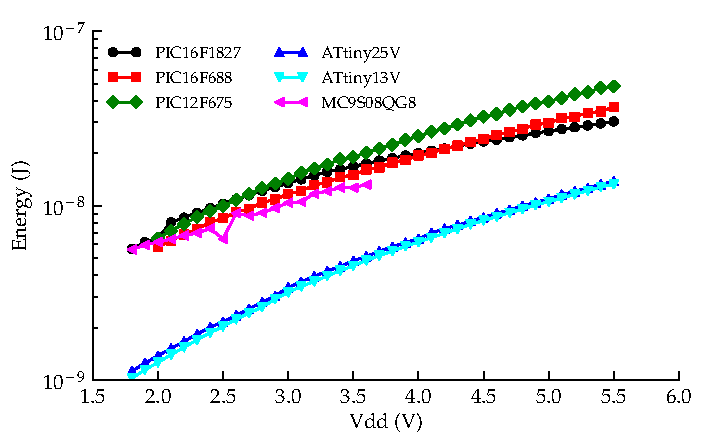
\includegraphics{content/pt1/02-Microcontrollers/graphics/Graph_ALL_ADC_JPM}
\protect\caption{Energy consumed by each MCU per ADC measurement.\label{fig:Energy-consumed-ADC}}

\par\end{centering}

\end{figure}


  
  \section{Data Transmission}
      
\section{Power Consumption}

\begin{figure}
\begin{centering}
\protect\caption{Power consumption of ZigBee}

\par\end{centering}

\end{figure}
\begin{figure}

\begin{centering}
\protect\caption{Power consumption of RFM12B}

\par\end{centering}

\end{figure}



\chapter{Discussion}

\chapter{Conclusion}